\documentclass[10pt]{article}
\usepackage[margin=1in]{geometry}
\usepackage[numbers,sort&compress]{natbib}
\usepackage{booktabs}
\usepackage{graphicx}
\usepackage{subcaption}
\usepackage{adjustbox}
\usepackage{amsmath}
\usepackage{microtype}
\usepackage[hidelinks]{hyperref}
\usepackage{xcolor}
\usepackage{caption}
\usepackage{enumitem}
\setlist{nosep,leftmargin=1.4em}
\captionsetup{font=small,labelfont=bf}
\renewcommand{\topfraction}{0.95}
\renewcommand{\bottomfraction}{0.9}
\renewcommand{\textfraction}{0.05}
\renewcommand{\floatpagefraction}{0.85}
\setcounter{topnumber}{3}
\setcounter{totalnumber}{5}

\graphicspath{{figs/}{../docs/img/}}
% generated by paper/make_tables.py from results/*.json; do not edit
\newcommand{\BRigDpGtfRawabsrel}{0.200}
\newcommand{\BRigDpGtfRawabsrelCI}{0.200 [0.178, 0.223]}
\newcommand{\BRigDpImgabsrel}{0.135}
\newcommand{\BRigDpImgabsrelCI}{0.135 [0.116, 0.161]}
\newcommand{\BRigDpImgdOne}{0.821}
\newcommand{\BRigDpImgrmse}{6.74}
\newcommand{\BRigDpRawabsrel}{0.188}
\newcommand{\BRigDpRawabsrelCI}{0.188 [0.166, 0.211]}
\newcommand{\BRigVggtImgabsrel}{0.124}
\newcommand{\BRigVggtImgabsrelCI}{0.124 [0.108, 0.140]}
\newcommand{\BRigVggtImgdOne}{0.854}
\newcommand{\BRigVggtImgrmse}{6.35}
\newcommand{\BRigVggtRawabsrel}{0.901}
\newcommand{\BRigVggtRawabsrelCI}{0.901 [0.898, 0.903]}
\newcommand{\BRigVggtSeqabsrel}{0.135}
\newcommand{\BRigVggtSeqabsrelCI}{0.135 [0.120, 0.149]}
\newcommand{\BRigVggtSeqdOne}{0.818}
\newcommand{\BRigVggtSeqrmse}{6.80}
\newcommand{\BRigVggtSimabsrel}{0.607}
\newcommand{\BRigVggtSimabsrelCI}{0.607 [0.517, 0.699]}
\newcommand{\BRigbaselineMean}{0.81}
\newcommand{\BRigfracVggtLower}{42}
\newcommand{\BRigminBaseline}{0.1}
\newcommand{\BRigmsPerSeq}{1333}
\newcommand{\BRignPairs}{200}
\newcommand{\BRignPairsBaseline}{200}
\newcommand{\BRignPairsExcluded}{0}
\newcommand{\BRignPoints}{120,040}
\newcommand{\BRignSeq}{40}
\newcommand{\BRigpairedImg}{-0.012 [-0.029, 0.003]}
\newcommand{\BRigpairedSeq}{-0.001 [-0.024, 0.017]}
\newcommand{\BRigpairedSeqMean}{-0.001}
\newcommand{\BRigrotMean}{8.12}
\newcommand{\BRigrotMedian}{4.65}
\newcommand{\BRigscaleSeqMedian}{23.4}
\newcommand{\BRigtransMean}{48.6}
\newcommand{\BRigtransMedian}{35.9}
\newcommand{\BTempDpGtfRawabsrel}{0.191}
\newcommand{\BTempDpGtfRawabsrelCI}{0.191 [0.170, 0.214]}
\newcommand{\BTempDpImgabsrel}{0.128}
\newcommand{\BTempDpImgabsrelCI}{0.128 [0.112, 0.151]}
\newcommand{\BTempDpImgdOne}{0.831}
\newcommand{\BTempDpImgrmse}{6.45}
\newcommand{\BTempDpRawabsrel}{0.186}
\newcommand{\BTempDpRawabsrelCI}{0.186 [0.162, 0.211]}
\newcommand{\BTempVggtImgabsrel}{0.123}
\newcommand{\BTempVggtImgabsrelCI}{0.123 [0.100, 0.153]}
\newcommand{\BTempVggtImgdOne}{0.862}
\newcommand{\BTempVggtImgrmse}{5.93}
\newcommand{\BTempVggtRawabsrel}{0.901}
\newcommand{\BTempVggtRawabsrelCI}{0.901 [0.898, 0.904]}
\newcommand{\BTempVggtSeqabsrel}{0.118}
\newcommand{\BTempVggtSeqabsrelCI}{0.118 [0.097, 0.146]}
\newcommand{\BTempVggtSeqdOne}{0.867}
\newcommand{\BTempVggtSeqrmse}{5.88}
\newcommand{\BTempVggtSimabsrel}{0.321}
\newcommand{\BTempVggtSimabsrelCI}{0.321 [0.208, 0.452]}
\newcommand{\BTempbaselineMean}{4.24}
\newcommand{\BTempfracVggtLower}{70}
\newcommand{\BTempminBaseline}{0.1}
\newcommand{\BTempmsPerSeq}{1192}
\newcommand{\BTempnPairs}{160}
\newcommand{\BTempnPairsBaseline}{120}
\newcommand{\BTempnPairsExcluded}{40}
\newcommand{\BTempnPoints}{120,495}
\newcommand{\BTempnSeq}{40}
\newcommand{\BTemppairedImg}{-0.005 [-0.020, 0.012]}
\newcommand{\BTemppairedSeq}{-0.010 [-0.026, 0.007]}
\newcommand{\BTemppairedSeqMean}{-0.010}
\newcommand{\BTemprotMean}{0.31}
\newcommand{\BTemprotMedian}{0.14}
\newcommand{\BTempscaleSeqMedian}{29.7}
\newcommand{\BTemptransMean}{2.3}
\newcommand{\BTemptransMedian}{2.0}
\newcommand{\DAVabsrelBackRaw}{1.034}
\newcommand{\DAVabsrelBackScaled}{0.191}
\newcommand{\DAVabsrelCamBackLeftRaw}{0.542}
\newcommand{\DAVabsrelCamBackLeftScaled}{0.190}
\newcommand{\DAVabsrelCamBackRaw}{1.034}
\newcommand{\DAVabsrelCamBackRightRaw}{0.412}
\newcommand{\DAVabsrelCamBackRightScaled}{0.223}
\newcommand{\DAVabsrelCamBackScaled}{0.191}
\newcommand{\DAVabsrelCamFrontLeftRaw}{0.514}
\newcommand{\DAVabsrelCamFrontLeftScaled}{0.202}
\newcommand{\DAVabsrelCamFrontRaw}{0.399}
\newcommand{\DAVabsrelCamFrontRightRaw}{0.432}
\newcommand{\DAVabsrelCamFrontRightScaled}{0.215}
\newcommand{\DAVabsrelCamFrontScaled}{0.140}
\newcommand{\DAVabsrelFarRaw}{0.250}
\newcommand{\DAVabsrelFarScaled}{0.405}
\newcommand{\DAVabsrelFrontRaw}{0.399}
\newcommand{\DAVabsrelFrontScaled}{0.140}
\newcommand{\DAVabsrelMidRaw}{0.334}
\newcommand{\DAVabsrelMidScaled}{0.238}
\newcommand{\DAVabsrelNearRaw}{0.668}
\newcommand{\DAVabsrelNearScaled}{0.168}
\newcommand{\DAVabsrelRaw}{0.582}
\newcommand{\DAVabsrelRawCI}{0.560 [0.549, 0.571]}
\newcommand{\DAVabsrelScaled}{0.194}
\newcommand{\DAVabsrelScaledCI}{0.193 [0.189, 0.197]}
\newcommand{\DAVabsrelSideRaw}{0.477}
\newcommand{\DAVabsrelSideScaled}{0.207}
\newcommand{\DAVbestGroup}{front}
\newcommand{\DAVdOneBackRaw}{0.097}
\newcommand{\DAVdOneBackScaled}{0.699}
\newcommand{\DAVdOneFrontRaw}{0.242}
\newcommand{\DAVdOneFrontScaled}{0.821}
\newcommand{\DAVdOneRaw}{0.199}
\newcommand{\DAVdOneScaled}{0.715}
\newcommand{\DAVdOneSideRaw}{0.222}
\newcommand{\DAVdOneSideScaled}{0.697}
\newcommand{\DAVdThreeRaw}{0.787}
\newcommand{\DAVdThreeScaled}{0.937}
\newcommand{\DAVfracAboveMax}{0.00}
\newcommand{\DAVimages}{2,424}
\newcommand{\DAVmsPerImage}{365}
\newcommand{\DAVpointsFar}{509,203}
\newcommand{\DAVpointsMid}{1,599,744}
\newcommand{\DAVpointsNear}{6,653,105}
\newcommand{\DAVrmseFarRaw}{16.98}
\newcommand{\DAVrmseFarScaled}{24.62}
\newcommand{\DAVrmseMidRaw}{12.10}
\newcommand{\DAVrmseMidScaled}{9.21}
\newcommand{\DAVrmseNearRaw}{6.96}
\newcommand{\DAVrmseNearScaled}{2.50}
\newcommand{\DAVrmseRaw}{8.96}
\newcommand{\DAVrmseScaled}{7.45}
\newcommand{\DAVrmselogRaw}{0.524}
\newcommand{\DAVrmselogScaled}{0.336}
\newcommand{\DAVscaleBack}{0.47}
\newcommand{\DAVscaleBackLeft}{0.68}
\newcommand{\DAVscaleBackLeftpNinety}{0.96}
\newcommand{\DAVscaleBackLeftpTen}{0.52}
\newcommand{\DAVscaleBackRight}{0.77}
\newcommand{\DAVscaleBackRightpNinety}{0.93}
\newcommand{\DAVscaleBackRightpTen}{0.61}
\newcommand{\DAVscaleBackpNinety}{0.56}
\newcommand{\DAVscaleBackpTen}{0.43}
\newcommand{\DAVscaleFront}{0.73}
\newcommand{\DAVscaleFrontLeft}{0.68}
\newcommand{\DAVscaleFrontLeftpNinety}{0.97}
\newcommand{\DAVscaleFrontLeftpTen}{0.57}
\newcommand{\DAVscaleFrontRight}{0.76}
\newcommand{\DAVscaleFrontRightpNinety}{0.92}
\newcommand{\DAVscaleFrontRightpTen}{0.63}
\newcommand{\DAVscaleFrontpNinety}{0.85}
\newcommand{\DAVscaleFrontpTen}{0.63}
\newcommand{\DAVscaleMax}{0.77}
\newcommand{\DAVscaleMin}{0.47}
\newcommand{\DAVscaleNonBackMax}{0.77}
\newcommand{\DAVscaleNonBackMin}{0.68}
\newcommand{\DAVscaleShare}{67}
\newcommand{\DAVsqrelRaw}{5.133}
\newcommand{\DAVsqrelScaled}{1.643}
\newcommand{\DAVwallMinutes}{14.9}
\newcommand{\DAVworstGroup}{back}
\newcommand{\DDPsteps}{20}
\newcommand{\DDPworld}{2}
\newcommand{\DPabsrelBackRaw}{0.259}
\newcommand{\DPabsrelBackScaled}{0.177}
\newcommand{\DPabsrelCamBackLeftRaw}{0.301}
\newcommand{\DPabsrelCamBackLeftScaled}{0.174}
\newcommand{\DPabsrelCamBackRaw}{0.259}
\newcommand{\DPabsrelCamBackRightRaw}{0.251}
\newcommand{\DPabsrelCamBackRightScaled}{0.202}
\newcommand{\DPabsrelCamBackScaled}{0.177}
\newcommand{\DPabsrelCamFrontLeftRaw}{0.286}
\newcommand{\DPabsrelCamFrontLeftScaled}{0.182}
\newcommand{\DPabsrelCamFrontRaw}{0.191}
\newcommand{\DPabsrelCamFrontRightRaw}{0.237}
\newcommand{\DPabsrelCamFrontRightScaled}{0.204}
\newcommand{\DPabsrelCamFrontScaled}{0.124}
\newcommand{\DPabsrelFarRaw}{0.373}
\newcommand{\DPabsrelFarScaled}{0.315}
\newcommand{\DPabsrelFrontRaw}{0.191}
\newcommand{\DPabsrelFrontScaled}{0.124}
\newcommand{\DPabsrelMidRaw}{0.280}
\newcommand{\DPabsrelMidScaled}{0.216}
\newcommand{\DPabsrelNearRaw}{0.242}
\newcommand{\DPabsrelNearScaled}{0.158}
\newcommand{\DPabsrelRaw}{0.257}
\newcommand{\DPabsrelRawCI}{0.255 [0.250, 0.260]}
\newcommand{\DPabsrelScaled}{0.178}
\newcommand{\DPabsrelScaledCI}{0.177 [0.173, 0.182]}
\newcommand{\DPabsrelSideRaw}{0.270}
\newcommand{\DPabsrelSideScaled}{0.190}
\newcommand{\DPbestGroup}{front}
\newcommand{\DPdOneBackRaw}{0.549}
\newcommand{\DPdOneBackScaled}{0.771}
\newcommand{\DPdOneFrontRaw}{0.633}
\newcommand{\DPdOneFrontScaled}{0.845}
\newcommand{\DPdOneRaw}{0.525}
\newcommand{\DPdOneScaled}{0.760}
\newcommand{\DPdOneSideRaw}{0.495}
\newcommand{\DPdOneSideScaled}{0.739}
\newcommand{\DPdThreeRaw}{0.894}
\newcommand{\DPdThreeScaled}{0.951}
\newcommand{\DPfocalPredBack}{1033}
\newcommand{\DPfocalPredBackLeft}{1366}
\newcommand{\DPfocalPredBackRight}{1415}
\newcommand{\DPfocalPredFront}{1324}
\newcommand{\DPfocalPredFrontLeft}{1322}
\newcommand{\DPfocalPredFrontRight}{1377}
\newcommand{\DPfocalRatioBack}{1.28}
\newcommand{\DPfocalRatioBackLeft}{1.09}
\newcommand{\DPfocalRatioBackRight}{1.12}
\newcommand{\DPfocalRatioFront}{1.05}
\newcommand{\DPfocalRatioFrontLeft}{1.04}
\newcommand{\DPfocalRatioFrontRight}{1.09}
\newcommand{\DPfocalRatioMax}{1.28}
\newcommand{\DPfocalRatioMin}{1.04}
\newcommand{\DPfocalTrueBack}{809}
\newcommand{\DPfocalTrueBackLeft}{1257}
\newcommand{\DPfocalTrueBackRight}{1260}
\newcommand{\DPfocalTrueFront}{1266}
\newcommand{\DPfocalTrueFrontLeft}{1273}
\newcommand{\DPfocalTrueFrontRight}{1261}
\newcommand{\DPfracAboveMax}{0.08}
\newcommand{\DPimages}{2,424}
\newcommand{\DPmsPerImage}{599}
\newcommand{\DPpointsFar}{509,203}
\newcommand{\DPpointsMid}{1,599,744}
\newcommand{\DPpointsNear}{6,653,105}
\newcommand{\DPrmseFarRaw}{23.38}
\newcommand{\DPrmseFarScaled}{20.43}
\newcommand{\DPrmseMidRaw}{10.22}
\newcommand{\DPrmseMidScaled}{8.81}
\newcommand{\DPrmseNearRaw}{3.52}
\newcommand{\DPrmseNearScaled}{2.99}
\newcommand{\DPrmseRaw}{7.76}
\newcommand{\DPrmseScaled}{6.73}
\newcommand{\DPrmselogRaw}{0.488}
\newcommand{\DPrmselogScaled}{0.314}
\newcommand{\DPscaleBack}{0.94}
\newcommand{\DPscaleBackLeft}{1.20}
\newcommand{\DPscaleBackLeftpNinety}{2.51}
\newcommand{\DPscaleBackLeftpTen}{0.93}
\newcommand{\DPscaleBackRight}{1.25}
\newcommand{\DPscaleBackRightpNinety}{1.64}
\newcommand{\DPscaleBackRightpTen}{1.02}
\newcommand{\DPscaleBackpNinety}{1.27}
\newcommand{\DPscaleBackpTen}{0.77}
\newcommand{\DPscaleFront}{1.12}
\newcommand{\DPscaleFrontLeft}{1.30}
\newcommand{\DPscaleFrontLeftpNinety}{1.97}
\newcommand{\DPscaleFrontLeftpTen}{1.02}
\newcommand{\DPscaleFrontRight}{1.21}
\newcommand{\DPscaleFrontRightpNinety}{1.70}
\newcommand{\DPscaleFrontRightpTen}{0.99}
\newcommand{\DPscaleFrontpNinety}{1.47}
\newcommand{\DPscaleFrontpTen}{0.88}
\newcommand{\DPscaleMax}{1.30}
\newcommand{\DPscaleMin}{0.94}
\newcommand{\DPscaleNonBackMax}{1.30}
\newcommand{\DPscaleNonBackMin}{1.12}
\newcommand{\DPscaleShare}{31}
\newcommand{\DPsqrelRaw}{2.123}
\newcommand{\DPsqrelScaled}{1.629}
\newcommand{\DPwallMinutes}{26.5}
\newcommand{\DPworstGroup}{side}
\newcommand{\DynVelThreshold}{0.5}
\newcommand{\FocalCheckDevice}{cpu fp32}
\newcommand{\FocalCheckMaxDiff}{0.0}
\newcommand{\GPUname}{NVIDIA L4}
\newcommand{\GSDepthHiFifteenKgaussians}{1,516,755}
\newcommand{\GSDepthHiFifteenKinitGaussians}{300,000}
\newcommand{\GSDepthHiFifteenKlpips}{0.417}
\newcommand{\GSDepthHiFifteenKnSeeds}{1}
\newcommand{\GSDepthHiFifteenKpsnr}{18.32}
\newcommand{\GSDepthHiFifteenKpsnrSeedMean}{18.32}
\newcommand{\GSDepthHiFifteenKpsnrSeedStd}{not measured}
\newcommand{\GSDepthHiFifteenKpsnrStd}{2.63}
\newcommand{\GSDepthHiFifteenKpsnrTrain}{23.32}
\newcommand{\GSDepthHiFifteenKrenderMs}{8.3}
\newcommand{\GSDepthHiFifteenKssim}{0.584}
\newcommand{\GSDepthHiFifteenKstepsPerS}{19.5}
\newcommand{\GSDepthHiFifteenKtrainMin}{12.8}
\newcommand{\GSDepthHigaussians}{736,227}
\newcommand{\GSDepthHiinitGaussians}{300,000}
\newcommand{\GSDepthHilpips}{0.497}
\newcommand{\GSDepthHinSeeds}{3}
\newcommand{\GSDepthHipsnr}{18.51}
\newcommand{\GSDepthHipsnrSeedMean}{18.43}
\newcommand{\GSDepthHipsnrSeedStd}{0.07}
\newcommand{\GSDepthHipsnrStd}{2.77}
\newcommand{\GSDepthHipsnrTrain}{21.48}
\newcommand{\GSDepthHirenderMs}{4.2}
\newcommand{\GSDepthHissim}{0.608}
\newcommand{\GSDepthHistepsPerS}{33.3}
\newcommand{\GSDepthHitrainMin}{3.5}
\newcommand{\GSDepthLoFifteenKgaussians}{1,337,190}
\newcommand{\GSDepthLoFifteenKinitGaussians}{300,000}
\newcommand{\GSDepthLoFifteenKlpips}{0.469}
\newcommand{\GSDepthLoFifteenKnSeeds}{1}
\newcommand{\GSDepthLoFifteenKpsnr}{16.94}
\newcommand{\GSDepthLoFifteenKpsnrSeedMean}{16.94}
\newcommand{\GSDepthLoFifteenKpsnrSeedStd}{not measured}
\newcommand{\GSDepthLoFifteenKpsnrStd}{2.79}
\newcommand{\GSDepthLoFifteenKpsnrTrain}{23.43}
\newcommand{\GSDepthLoFifteenKrenderMs}{7.2}
\newcommand{\GSDepthLoFifteenKssim}{0.574}
\newcommand{\GSDepthLoFifteenKstepsPerS}{21.6}
\newcommand{\GSDepthLoFifteenKtrainMin}{11.6}
\newcommand{\GSDepthLogaussians}{674,323}
\newcommand{\GSDepthLoinitGaussians}{300,000}
\newcommand{\GSDepthLolpips}{0.525}
\newcommand{\GSDepthLonSeeds}{3}
\newcommand{\GSDepthLopsnr}{17.54}
\newcommand{\GSDepthLopsnrSeedMean}{17.46}
\newcommand{\GSDepthLopsnrSeedStd}{0.10}
\newcommand{\GSDepthLopsnrStd}{2.66}
\newcommand{\GSDepthLopsnrTrain}{21.66}
\newcommand{\GSDepthLorenderMs}{3.9}
\newcommand{\GSDepthLossim}{0.599}
\newcommand{\GSDepthLostepsPerS}{35.0}
\newcommand{\GSDepthLotrainMin}{3.3}
\newcommand{\GSLidarFifteenKgaussians}{948,796}
\newcommand{\GSLidarFifteenKinitGaussians}{300,000}
\newcommand{\GSLidarFifteenKlpips}{0.605}
\newcommand{\GSLidarFifteenKnSeeds}{1}
\newcommand{\GSLidarFifteenKpsnr}{14.04}
\newcommand{\GSLidarFifteenKpsnrSeedMean}{14.04}
\newcommand{\GSLidarFifteenKpsnrSeedStd}{not measured}
\newcommand{\GSLidarFifteenKpsnrStd}{3.42}
\newcommand{\GSLidarFifteenKpsnrTrain}{22.44}
\newcommand{\GSLidarFifteenKrenderMs}{5.0}
\newcommand{\GSLidarFifteenKssim}{0.522}
\newcommand{\GSLidarFifteenKstepsPerS}{29.7}
\newcommand{\GSLidarFifteenKtrainMin}{8.4}
\newcommand{\GSLidargaussians}{576,114}
\newcommand{\GSLidarinitGaussians}{300,000}
\newcommand{\GSLidarlpips}{0.580}
\newcommand{\GSLidarnSeeds}{3}
\newcommand{\GSLidarpsnr}{16.29}
\newcommand{\GSLidarpsnrSeedMean}{15.91}
\newcommand{\GSLidarpsnrSeedStd}{0.37}
\newcommand{\GSLidarpsnrStd}{2.75}
\newcommand{\GSLidarpsnrTrain}{21.24}
\newcommand{\GSLidarrenderMs}{3.5}
\newcommand{\GSLidarssim}{0.587}
\newcommand{\GSLidarstepsPerS}{40.1}
\newcommand{\GSLidartrainMin}{2.9}
\newcommand{\GSRandFifteenKgaussians}{427,153}
\newcommand{\GSRandFifteenKinitGaussians}{200,000}
\newcommand{\GSRandFifteenKlpips}{0.729}
\newcommand{\GSRandFifteenKnSeeds}{1}
\newcommand{\GSRandFifteenKpsnr}{12.36}
\newcommand{\GSRandFifteenKpsnrSeedMean}{12.36}
\newcommand{\GSRandFifteenKpsnrSeedStd}{not measured}
\newcommand{\GSRandFifteenKpsnrStd}{2.45}
\newcommand{\GSRandFifteenKpsnrTrain}{20.61}
\newcommand{\GSRandFifteenKrenderMs}{2.6}
\newcommand{\GSRandFifteenKssim}{0.512}
\newcommand{\GSRandFifteenKstepsPerS}{56.2}
\newcommand{\GSRandFifteenKtrainMin}{4.4}
\newcommand{\GSRandgaussians}{206,811}
\newcommand{\GSRandinitGaussians}{200,000}
\newcommand{\GSRandlpips}{0.758}
\newcommand{\GSRandnSeeds}{3}
\newcommand{\GSRandpsnr}{13.40}
\newcommand{\GSRandpsnrSeedMean}{13.78}
\newcommand{\GSRandpsnrSeedStd}{0.42}
\newcommand{\GSRandpsnrStd}{3.78}
\newcommand{\GSRandpsnrTrain}{20.01}
\newcommand{\GSRandrenderMs}{1.9}
\newcommand{\GSRandssim}{0.521}
\newcommand{\GSRandstepsPerS}{77.7}
\newcommand{\GSRandtrainMin}{1.5}
\newcommand{\GSdeltaDepthHiLpips}{-0.083}
\newcommand{\GSdeltaDepthHiLpipsFifteenK}{-0.188}
\newcommand{\GSdeltaDepthHiPsnr}{2.22}
\newcommand{\GSdeltaDepthHiPsnrFifteenK}{4.28}
\newcommand{\GSdeltaDepthLoLpips}{-0.054}
\newcommand{\GSdeltaDepthLoLpipsFifteenK}{-0.136}
\newcommand{\GSdeltaDepthLoPsnr}{1.26}
\newcommand{\GSdeltaDepthLoPsnrFifteenK}{2.90}
\newcommand{\GSdeltaLidarRandom}{2.89}
\newcommand{\GSdeltaLidarRandomFifteenK}{1.68}
\newcommand{\GSdownscale}{2}
\newcommand{\GSholdout}{every 8th timestamp (offset 4), all 6 cameras}
\newcommand{\GSimageH}{450}
\newcommand{\GSimageW}{800}
\newcommand{\GSnSeeds}{3}
\newcommand{\GSscene}{scene-0916}
\newcommand{\GSsceneAnnotations}{2,424}
\newcommand{\GSsceneFracMoving}{8}
\newcommand{\GSsceneKeyframes}{41}
\newcommand{\GSsceneMoving}{186}
\newcommand{\GSseedCaption}{The seed columns give mean $\pm$ sample standard deviation of the per-run means over the seeds that were run (n in brackets).}
\newcommand{\GSseedSentence}{Seeds 0, 1, 2 were run for the variants marked in Table~\ref{tab:track_c}; the seed column reports mean and sample standard deviation over seeds.}
\newcommand{\GSseedStatus}{measured}
\newcommand{\GStestViews}{30}
\newcommand{\GStrainViews}{216}
\newcommand{\GTFabsrelBackRaw}{0.236}
\newcommand{\GTFabsrelBackScaled}{0.177}
\newcommand{\GTFabsrelCamBackLeftRaw}{0.326}
\newcommand{\GTFabsrelCamBackLeftScaled}{0.174}
\newcommand{\GTFabsrelCamBackRaw}{0.236}
\newcommand{\GTFabsrelCamBackRightRaw}{0.309}
\newcommand{\GTFabsrelCamBackRightScaled}{0.202}
\newcommand{\GTFabsrelCamBackScaled}{0.177}
\newcommand{\GTFabsrelCamFrontLeftRaw}{0.310}
\newcommand{\GTFabsrelCamFrontLeftScaled}{0.182}
\newcommand{\GTFabsrelCamFrontRaw}{0.202}
\newcommand{\GTFabsrelCamFrontRightRaw}{0.275}
\newcommand{\GTFabsrelCamFrontRightScaled}{0.204}
\newcommand{\GTFabsrelCamFrontScaled}{0.124}
\newcommand{\GTFabsrelFarRaw}{0.438}
\newcommand{\GTFabsrelFarScaled}{0.315}
\newcommand{\GTFabsrelFrontRaw}{0.202}
\newcommand{\GTFabsrelFrontScaled}{0.124}
\newcommand{\GTFabsrelMidRaw}{0.338}
\newcommand{\GTFabsrelMidScaled}{0.216}
\newcommand{\GTFabsrelNearRaw}{0.250}
\newcommand{\GTFabsrelNearScaled}{0.158}
\newcommand{\GTFabsrelRaw}{0.277}
\newcommand{\GTFabsrelRawCI}{0.276 [0.271, 0.282]}
\newcommand{\GTFabsrelScaled}{0.178}
\newcommand{\GTFabsrelScaledCI}{0.177 [0.173, 0.182]}
\newcommand{\GTFabsrelSideRaw}{0.306}
\newcommand{\GTFabsrelSideScaled}{0.190}
\newcommand{\GTFbestGroup}{front}
\newcommand{\GTFdOneBackRaw}{0.525}
\newcommand{\GTFdOneBackScaled}{0.771}
\newcommand{\GTFdOneFrontRaw}{0.595}
\newcommand{\GTFdOneFrontScaled}{0.845}
\newcommand{\GTFdOneRaw}{0.460}
\newcommand{\GTFdOneScaled}{0.760}
\newcommand{\GTFdOneSideRaw}{0.411}
\newcommand{\GTFdOneSideScaled}{0.739}
\newcommand{\GTFdThreeRaw}{0.858}
\newcommand{\GTFdThreeScaled}{0.951}
\newcommand{\GTFfocalPredBack}{1033}
\newcommand{\GTFfocalPredBackLeft}{1366}
\newcommand{\GTFfocalPredBackRight}{1415}
\newcommand{\GTFfocalPredFront}{1324}
\newcommand{\GTFfocalPredFrontLeft}{1322}
\newcommand{\GTFfocalPredFrontRight}{1377}
\newcommand{\GTFfocalRatioBack}{1.28}
\newcommand{\GTFfocalRatioBackLeft}{1.09}
\newcommand{\GTFfocalRatioBackRight}{1.12}
\newcommand{\GTFfocalRatioFront}{1.05}
\newcommand{\GTFfocalRatioFrontLeft}{1.04}
\newcommand{\GTFfocalRatioFrontRight}{1.09}
\newcommand{\GTFfocalRatioMax}{1.28}
\newcommand{\GTFfocalRatioMin}{1.04}
\newcommand{\GTFfocalTrueBack}{809}
\newcommand{\GTFfocalTrueBackLeft}{1257}
\newcommand{\GTFfocalTrueBackRight}{1260}
\newcommand{\GTFfocalTrueFront}{1266}
\newcommand{\GTFfocalTrueFrontLeft}{1273}
\newcommand{\GTFfocalTrueFrontRight}{1261}
\newcommand{\GTFfracAboveMax}{0.06}
\newcommand{\GTFimages}{2,424}
\newcommand{\GTFmsPerImage}{599}
\newcommand{\GTFpointsFar}{509,203}
\newcommand{\GTFpointsMid}{1,599,744}
\newcommand{\GTFpointsNear}{6,653,105}
\newcommand{\GTFrmseFarRaw}{26.08}
\newcommand{\GTFrmseFarScaled}{20.43}
\newcommand{\GTFrmseMidRaw}{11.55}
\newcommand{\GTFrmseMidScaled}{8.81}
\newcommand{\GTFrmseNearRaw}{3.58}
\newcommand{\GTFrmseNearScaled}{2.99}
\newcommand{\GTFrmseRaw}{8.58}
\newcommand{\GTFrmseScaled}{6.73}
\newcommand{\GTFrmselogRaw}{0.553}
\newcommand{\GTFrmselogScaled}{0.314}
\newcommand{\GTFscaleBack}{1.17}
\newcommand{\GTFscaleBackLeft}{1.27}
\newcommand{\GTFscaleBackLeftpNinety}{3.17}
\newcommand{\GTFscaleBackLeftpTen}{1.06}
\newcommand{\GTFscaleBackRight}{1.39}
\newcommand{\GTFscaleBackRightpNinety}{2.07}
\newcommand{\GTFscaleBackRightpTen}{1.08}
\newcommand{\GTFscaleBackpNinety}{1.57}
\newcommand{\GTFscaleBackpTen}{1.01}
\newcommand{\GTFscaleFront}{1.16}
\newcommand{\GTFscaleFrontLeft}{1.34}
\newcommand{\GTFscaleFrontLeftpNinety}{2.18}
\newcommand{\GTFscaleFrontLeftpTen}{1.07}
\newcommand{\GTFscaleFrontRight}{1.29}
\newcommand{\GTFscaleFrontRightpNinety}{2.01}
\newcommand{\GTFscaleFrontRightpTen}{1.07}
\newcommand{\GTFscaleFrontpNinety}{1.53}
\newcommand{\GTFscaleFrontpTen}{0.95}
\newcommand{\GTFscaleMax}{1.39}
\newcommand{\GTFscaleMin}{1.16}
\newcommand{\GTFscaleNonBackMax}{1.39}
\newcommand{\GTFscaleNonBackMin}{1.16}
\newcommand{\GTFscaleShare}{36}
\newcommand{\GTFsqrelRaw}{2.448}
\newcommand{\GTFsqrelScaled}{1.629}
\newcommand{\GTFwallMinutes}{26.5}
\newcommand{\GTFworstGroup}{side}
\newcommand{\GTfracNearMax}{87}
\newcommand{\GTfracNearMin}{69}
\newcommand{\GTimages}{2,424}
\newcommand{\GTkeyframes}{404}
\newcommand{\GTmedianZmax}{11.9}
\newcommand{\GTmedianZmin}{8.4}
\newcommand{\GTptsMax}{4521}
\newcommand{\GTptsMin}{3020}
\newcommand{\GTwallSeconds}{27}
\newcommand{\MOGEGTFabsrelBackRaw}{0.190}
\newcommand{\MOGEGTFabsrelBackScaled}{0.134}
\newcommand{\MOGEGTFabsrelCamBackLeftRaw}{0.189}
\newcommand{\MOGEGTFabsrelCamBackLeftScaled}{0.150}
\newcommand{\MOGEGTFabsrelCamBackRaw}{0.190}
\newcommand{\MOGEGTFabsrelCamBackRightRaw}{0.153}
\newcommand{\MOGEGTFabsrelCamBackRightScaled}{0.166}
\newcommand{\MOGEGTFabsrelCamBackScaled}{0.134}
\newcommand{\MOGEGTFabsrelCamFrontLeftRaw}{0.175}
\newcommand{\MOGEGTFabsrelCamFrontLeftScaled}{0.163}
\newcommand{\MOGEGTFabsrelCamFrontRaw}{0.128}
\newcommand{\MOGEGTFabsrelCamFrontRightRaw}{0.161}
\newcommand{\MOGEGTFabsrelCamFrontRightScaled}{0.178}
\newcommand{\MOGEGTFabsrelCamFrontScaled}{0.123}
\newcommand{\MOGEGTFabsrelFarRaw}{0.243}
\newcommand{\MOGEGTFabsrelFarScaled}{0.261}
\newcommand{\MOGEGTFabsrelFrontRaw}{0.128}
\newcommand{\MOGEGTFabsrelFrontScaled}{0.123}
\newcommand{\MOGEGTFabsrelMidRaw}{0.190}
\newcommand{\MOGEGTFabsrelMidScaled}{0.189}
\newcommand{\MOGEGTFabsrelNearRaw}{0.158}
\newcommand{\MOGEGTFabsrelNearScaled}{0.134}
\newcommand{\MOGEGTFabsrelRaw}{0.168}
\newcommand{\MOGEGTFabsrelRawCI}{0.166 [0.163, 0.169]}
\newcommand{\MOGEGTFabsrelScaled}{0.152}
\newcommand{\MOGEGTFabsrelScaledCI}{0.153 [0.148, 0.157]}
\newcommand{\MOGEGTFabsrelSideRaw}{0.170}
\newcommand{\MOGEGTFabsrelSideScaled}{0.164}
\newcommand{\MOGEGTFbestGroup}{front}
\newcommand{\MOGEGTFdOneBackRaw}{0.769}
\newcommand{\MOGEGTFdOneBackScaled}{0.847}
\newcommand{\MOGEGTFdOneFrontRaw}{0.889}
\newcommand{\MOGEGTFdOneFrontScaled}{0.860}
\newcommand{\MOGEGTFdOneRaw}{0.812}
\newcommand{\MOGEGTFdOneScaled}{0.812}
\newcommand{\MOGEGTFdOneSideRaw}{0.809}
\newcommand{\MOGEGTFdOneSideScaled}{0.790}
\newcommand{\MOGEGTFdThreeRaw}{0.953}
\newcommand{\MOGEGTFdThreeScaled}{0.957}
\newcommand{\MOGEGTFfocalPredBack}{991}
\newcommand{\MOGEGTFfocalPredBackLeft}{1269}
\newcommand{\MOGEGTFfocalPredBackRight}{1249}
\newcommand{\MOGEGTFfocalPredFront}{1214}
\newcommand{\MOGEGTFfocalPredFrontLeft}{1239}
\newcommand{\MOGEGTFfocalPredFrontRight}{1259}
\newcommand{\MOGEGTFfocalRatioBack}{1.22}
\newcommand{\MOGEGTFfocalRatioBackLeft}{1.01}
\newcommand{\MOGEGTFfocalRatioBackRight}{0.99}
\newcommand{\MOGEGTFfocalRatioFront}{0.96}
\newcommand{\MOGEGTFfocalRatioFrontLeft}{0.97}
\newcommand{\MOGEGTFfocalRatioFrontRight}{1.00}
\newcommand{\MOGEGTFfocalRatioMax}{1.22}
\newcommand{\MOGEGTFfocalRatioMin}{0.96}
\newcommand{\MOGEGTFfocalTrueBack}{809}
\newcommand{\MOGEGTFfocalTrueBackLeft}{1257}
\newcommand{\MOGEGTFfocalTrueBackRight}{1260}
\newcommand{\MOGEGTFfocalTrueFront}{1266}
\newcommand{\MOGEGTFfocalTrueFrontLeft}{1273}
\newcommand{\MOGEGTFfocalTrueFrontRight}{1261}
\newcommand{\MOGEGTFfracAboveMax}{0.09}
\newcommand{\MOGEGTFimages}{2,424}
\newcommand{\MOGEGTFmsPerImage}{188}
\newcommand{\MOGEGTFpointsFar}{509,203}
\newcommand{\MOGEGTFpointsMid}{1,599,744}
\newcommand{\MOGEGTFpointsNear}{6,653,105}
\newcommand{\MOGEGTFrmseFarRaw}{17.57}
\newcommand{\MOGEGTFrmseFarScaled}{18.29}
\newcommand{\MOGEGTFrmseMidRaw}{8.11}
\newcommand{\MOGEGTFrmseMidScaled}{8.29}
\newcommand{\MOGEGTFrmseNearRaw}{2.62}
\newcommand{\MOGEGTFrmseNearScaled}{2.51}
\newcommand{\MOGEGTFrmseRaw}{5.93}
\newcommand{\MOGEGTFrmseScaled}{6.06}
\newcommand{\MOGEGTFrmselogRaw}{0.308}
\newcommand{\MOGEGTFrmselogScaled}{0.293}
\newcommand{\MOGEGTFscaleBack}{0.92}
\newcommand{\MOGEGTFscaleBackLeft}{0.99}
\newcommand{\MOGEGTFscaleBackLeftpNinety}{1.14}
\newcommand{\MOGEGTFscaleBackLeftpTen}{0.86}
\newcommand{\MOGEGTFscaleBackRight}{0.97}
\newcommand{\MOGEGTFscaleBackRightpNinety}{1.16}
\newcommand{\MOGEGTFscaleBackRightpTen}{0.88}
\newcommand{\MOGEGTFscaleBackpNinety}{1.02}
\newcommand{\MOGEGTFscaleBackpTen}{0.80}
\newcommand{\MOGEGTFscaleFront}{0.98}
\newcommand{\MOGEGTFscaleFrontLeft}{0.97}
\newcommand{\MOGEGTFscaleFrontLeftpNinety}{1.22}
\newcommand{\MOGEGTFscaleFrontLeftpTen}{0.87}
\newcommand{\MOGEGTFscaleFrontRight}{0.98}
\newcommand{\MOGEGTFscaleFrontRightpNinety}{1.17}
\newcommand{\MOGEGTFscaleFrontRightpTen}{0.89}
\newcommand{\MOGEGTFscaleFrontpNinety}{1.10}
\newcommand{\MOGEGTFscaleFrontpTen}{0.88}
\newcommand{\MOGEGTFscaleMax}{0.99}
\newcommand{\MOGEGTFscaleMin}{0.92}
\newcommand{\MOGEGTFscaleNonBackMax}{0.99}
\newcommand{\MOGEGTFscaleNonBackMin}{0.97}
\newcommand{\MOGEGTFscaleShare}{10}
\newcommand{\MOGEGTFsqrelRaw}{1.258}
\newcommand{\MOGEGTFsqrelScaled}{1.280}
\newcommand{\MOGEGTFwallMinutes}{8.0}
\newcommand{\MOGEGTFworstGroup}{back}
\newcommand{\MOGEabsrelBackRaw}{0.289}
\newcommand{\MOGEabsrelBackScaled}{0.140}
\newcommand{\MOGEabsrelCamBackLeftRaw}{0.195}
\newcommand{\MOGEabsrelCamBackLeftScaled}{0.152}
\newcommand{\MOGEabsrelCamBackRaw}{0.289}
\newcommand{\MOGEabsrelCamBackRightRaw}{0.169}
\newcommand{\MOGEabsrelCamBackRightScaled}{0.164}
\newcommand{\MOGEabsrelCamBackScaled}{0.140}
\newcommand{\MOGEabsrelCamFrontLeftRaw}{0.169}
\newcommand{\MOGEabsrelCamFrontLeftScaled}{0.161}
\newcommand{\MOGEabsrelCamFrontRaw}{0.122}
\newcommand{\MOGEabsrelCamFrontRightRaw}{0.175}
\newcommand{\MOGEabsrelCamFrontRightScaled}{0.179}
\newcommand{\MOGEabsrelCamFrontScaled}{0.112}
\newcommand{\MOGEabsrelFarRaw}{0.244}
\newcommand{\MOGEabsrelFarScaled}{0.265}
\newcommand{\MOGEabsrelFrontRaw}{0.122}
\newcommand{\MOGEabsrelFrontScaled}{0.112}
\newcommand{\MOGEabsrelMidRaw}{0.198}
\newcommand{\MOGEabsrelMidScaled}{0.189}
\newcommand{\MOGEabsrelNearRaw}{0.188}
\newcommand{\MOGEabsrelNearScaled}{0.133}
\newcommand{\MOGEabsrelRaw}{0.193}
\newcommand{\MOGEabsrelRawCI}{0.187 [0.183, 0.190]}
\newcommand{\MOGEabsrelScaled}{0.151}
\newcommand{\MOGEabsrelScaledCI}{0.151 [0.147, 0.156]}
\newcommand{\MOGEabsrelSideRaw}{0.178}
\newcommand{\MOGEabsrelSideScaled}{0.163}
\newcommand{\MOGEbestGroup}{front}
\newcommand{\MOGEdOneBackRaw}{0.493}
\newcommand{\MOGEdOneBackScaled}{0.843}
\newcommand{\MOGEdOneFrontRaw}{0.860}
\newcommand{\MOGEdOneFrontScaled}{0.880}
\newcommand{\MOGEdOneRaw}{0.731}
\newcommand{\MOGEdOneScaled}{0.813}
\newcommand{\MOGEdOneSideRaw}{0.779}
\newcommand{\MOGEdOneSideScaled}{0.790}
\newcommand{\MOGEdThreeRaw}{0.955}
\newcommand{\MOGEdThreeScaled}{0.956}
\newcommand{\MOGEfocalPredBack}{991}
\newcommand{\MOGEfocalPredBackLeft}{1269}
\newcommand{\MOGEfocalPredBackRight}{1249}
\newcommand{\MOGEfocalPredFront}{1214}
\newcommand{\MOGEfocalPredFrontLeft}{1239}
\newcommand{\MOGEfocalPredFrontRight}{1259}
\newcommand{\MOGEfocalRatioBack}{1.22}
\newcommand{\MOGEfocalRatioBackLeft}{1.01}
\newcommand{\MOGEfocalRatioBackRight}{0.99}
\newcommand{\MOGEfocalRatioFront}{0.96}
\newcommand{\MOGEfocalRatioFrontLeft}{0.97}
\newcommand{\MOGEfocalRatioFrontRight}{1.00}
\newcommand{\MOGEfocalRatioMax}{1.22}
\newcommand{\MOGEfocalRatioMin}{0.96}
\newcommand{\MOGEfocalTrueBack}{809}
\newcommand{\MOGEfocalTrueBackLeft}{1257}
\newcommand{\MOGEfocalTrueBackRight}{1260}
\newcommand{\MOGEfocalTrueFront}{1266}
\newcommand{\MOGEfocalTrueFrontLeft}{1273}
\newcommand{\MOGEfocalTrueFrontRight}{1261}
\newcommand{\MOGEfracAboveMax}{0.10}
\newcommand{\MOGEimages}{2,424}
\newcommand{\MOGEmsPerImage}{188}
\newcommand{\MOGEpointsFar}{509,203}
\newcommand{\MOGEpointsMid}{1,599,744}
\newcommand{\MOGEpointsNear}{6,653,105}
\newcommand{\MOGErmseFarRaw}{17.56}
\newcommand{\MOGErmseFarScaled}{18.46}
\newcommand{\MOGErmseMidRaw}{8.22}
\newcommand{\MOGErmseMidScaled}{8.28}
\newcommand{\MOGErmseNearRaw}{2.82}
\newcommand{\MOGErmseNearScaled}{2.49}
\newcommand{\MOGErmseRaw}{6.03}
\newcommand{\MOGErmseScaled}{6.09}
\newcommand{\MOGErmselogRaw}{0.316}
\newcommand{\MOGErmselogScaled}{0.292}
\newcommand{\MOGEscaleBack}{0.85}
\newcommand{\MOGEscaleBackLeft}{0.98}
\newcommand{\MOGEscaleBackLeftpNinety}{1.12}
\newcommand{\MOGEscaleBackLeftpTen}{0.84}
\newcommand{\MOGEscaleBackRight}{0.99}
\newcommand{\MOGEscaleBackRightpNinety}{1.18}
\newcommand{\MOGEscaleBackRightpTen}{0.86}
\newcommand{\MOGEscaleBackpNinety}{0.94}
\newcommand{\MOGEscaleBackpTen}{0.73}
\newcommand{\MOGEscaleFront}{1.01}
\newcommand{\MOGEscaleFrontLeft}{0.99}
\newcommand{\MOGEscaleFrontLeftpNinety}{1.21}
\newcommand{\MOGEscaleFrontLeftpTen}{0.89}
\newcommand{\MOGEscaleFrontRight}{0.99}
\newcommand{\MOGEscaleFrontRightpNinety}{1.17}
\newcommand{\MOGEscaleFrontRightpTen}{0.85}
\newcommand{\MOGEscaleFrontpNinety}{1.18}
\newcommand{\MOGEscaleFrontpTen}{0.90}
\newcommand{\MOGEscaleMax}{1.01}
\newcommand{\MOGEscaleMin}{0.85}
\newcommand{\MOGEscaleNonBackMax}{1.01}
\newcommand{\MOGEscaleNonBackMin}{0.98}
\newcommand{\MOGEscaleShare}{22}
\newcommand{\MOGEsqrelRaw}{1.366}
\newcommand{\MOGEsqrelScaled}{1.277}
\newcommand{\MOGEwallMinutes}{8.0}
\newcommand{\MOGEworstGroup}{back}
\newcommand{\MoGeAbstract}{ MoGe-2 has raw AbsRel 0.193 and 0.151 after scaling, and with the true focal its raw AbsRel is 0.168 (lower than with its own estimate).}
\newcommand{\MoGeDiscussion}{MoGe-2 does not show this effect: the true focal lowers its raw AbsRel from 0.193 to 0.168.}
\newcommand{\MoGeResults}{MoGe-2 has raw AbsRel 0.193 and 0.151 after median scaling, so 22\% of its raw error is a per-image scale error; its median scale factors per camera lie between 0.85 and 1.01. With the true focal length its raw AbsRel is 0.168, lower than with its own focal estimate, and the scale factors lie between 0.92 and 0.99. Its focal estimate is 0.96 to 1.22 times the true focal. Ordered by raw AbsRel the own-focal variants are MoGe-2 $<$ Depth Pro $<$ Depth Anything V2; ordered by median-scaled AbsRel they are MoGe-2 $<$ Depth Pro $<$ Depth Anything V2. MoGe-2 takes 188 ms per image on the NVIDIA L4 (median).}
\newcommand{\MoGeRowNote}{}
\newcommand{\MoGeScaleShape}{MoGe-2 has the smallest scale share of the three (22\%) and a median-scaled AbsRel of 0.151.}
\newcommand{\MoGeSentence}{MoGe-2 was run with the same protocol, with its own focal estimate and with the true focal length.}
\newcommand{\MoGeStatus}{measured}
\newcommand{\NFCopylpips}{0.040}
\newcommand{\NFCopylpipsCI}{0.040 [0.038, 0.042]}
\newcommand{\NFCopylpipsSeedMean}{0.040}
\newcommand{\NFCopylpipsSeedStd}{0.000}
\newcommand{\NFCopypsnr}{24.38}
\newcommand{\NFCopypsnrCI}{24.38 [24.09, 24.69]}
\newcommand{\NFCopypsnrSeedMean}{24.38}
\newcommand{\NFCopypsnrSeedStd}{0.00}
\newcommand{\NFFmbatch}{64}
\newcommand{\NFFmfinalLoss}{0.0430}
\newcommand{\NFFmlpips}{0.099}
\newcommand{\NFFmlpipsCI}{0.099 [0.096, 0.102]}
\newcommand{\NFFmlpipsSeedMean}{0.098}
\newcommand{\NFFmlpipsSeedStd}{0.006}
\newcommand{\NFFmlr}{0.0002}
\newcommand{\NFFmmaxMinutes}{40}
\newcommand{\NFFmparams}{12.4}
\newcommand{\NFFmpsnr}{23.82}
\newcommand{\NFFmpsnrCI}{23.82 [23.61, 24.04]}
\newcommand{\NFFmpsnrSeedMean}{23.80}
\newcommand{\NFFmpsnrSeedStd}{0.10}
\newcommand{\NFFmsteps}{2,150}
\newcommand{\NFFmstepsPerS}{0.9}
\newcommand{\NFFmstepsRequested}{12,000}
\newcommand{\NFFmtrainMin}{40.0}
\newcommand{\NFRegbatch}{64}
\newcommand{\NFRegfinalLoss}{0.0025}
\newcommand{\NFReglpips}{0.121}
\newcommand{\NFReglpipsCI}{0.121 [0.119, 0.123]}
\newcommand{\NFReglpipsSeedMean}{0.120}
\newcommand{\NFReglpipsSeedStd}{0.003}
\newcommand{\NFReglr}{0.0002}
\newcommand{\NFRegmaxMinutes}{40}
\newcommand{\NFRegparams}{12.4}
\newcommand{\NFRegpsnr}{24.74}
\newcommand{\NFRegpsnrCI}{24.74 [24.52, 24.98]}
\newcommand{\NFRegpsnrSeedMean}{24.92}
\newcommand{\NFRegpsnrSeedStd}{0.19}
\newcommand{\NFRegsteps}{2,150}
\newcommand{\NFRegstepsPerS}{0.9}
\newcommand{\NFRegstepsRequested}{12,000}
\newcommand{\NFRegtrainMin}{40.0}
\newcommand{\NFdtMedian}{0.10}
\newcommand{\NFfid}{390.3}
\newcommand{\NFfidN}{467}
\newcommand{\NFfracFmLowerReg}{73}
\newcommand{\NFframes}{2,342}
\newcommand{\NFh}{64}
\newcommand{\NFholdoutScenes}{scene-0655, scene-1094}
\newcommand{\NFkeyframes}{404}
\newcommand{\NFnSeeds}{3}
\newcommand{\NFpairedLpipsFmCopy}{0.059 [0.057, 0.061]}
\newcommand{\NFpairedLpipsFmReg}{-0.022 [-0.025, -0.019]}
\newcommand{\NFpairedLpipsFmRegMean}{-0.022}
\newcommand{\NFpairedPsnrFmCopy}{-0.56 [-0.73, -0.40]}
\newcommand{\NFsampler}{Euler, 50 steps}
\newcommand{\NFsamplingMs}{173.8}
\newcommand{\NFseedCaption}{The seed columns give mean $\pm$ sample standard deviation of the per-run means over seeds.}
\newcommand{\NFseedSentence}{Seeds 0, 1, 2 (training and sampling seed) were run; Table~\ref{tab:track_e} adds mean and sample standard deviation over seeds.}
\newcommand{\NFseedStatus}{measured}
\newcommand{\NFtestPairs}{467}
\newcommand{\NFtrainPairs}{1,865}
\newcommand{\NFw}{128}
\newcommand{\PPsentence}{the calibrated nuScenes principal points are on average 22 px (horizontal) and 30 px (vertical) away from the centre of the 1600x900 images, at most 58 px}
\newcommand{\SharpDtKeyframe}{0.50}
\newcommand{\SharpEvalH}{450}
\newcommand{\SharpEvalW}{800}
\newcommand{\SharpGaussiansMax}{1,179,648}
\newcommand{\SharpGaussiansMin}{1,179,648}
\newcommand{\SharpIdcoverage}{1.00}
\newcommand{\SharpIdlpips}{0.017}
\newcommand{\SharpIdlpipsCI}{0.017 [0.014, 0.020]}
\newcommand{\SharpIdmotion}{0.00}
\newcommand{\SharpIdpsnr}{41.62}
\newcommand{\SharpIdpsnrCI}{41.62 [40.69, 42.52]}
\newcommand{\SharpIdssim}{0.991}
\newcommand{\SharpImages}{10}
\newcommand{\SharpKeycoverage}{1.00}
\newcommand{\SharpKeylpips}{0.231}
\newcommand{\SharpKeylpipsCI}{0.231 [0.179, 0.290]}
\newcommand{\SharpKeymotion}{2.82}
\newcommand{\SharpKeypsnr}{20.42}
\newcommand{\SharpKeypsnrCI}{20.42 [18.71, 22.09]}
\newcommand{\SharpKeyssim}{0.592}
\newcommand{\SharpModelLoadSeconds}{10}
\newcommand{\SharpPredictMs}{5496}
\newcommand{\SharpRenderMs}{22.0}
\newcommand{\SharpSweepcoverage}{1.00}
\newcommand{\SharpSweeplpips}{0.096}
\newcommand{\SharpSweeplpipsCI}{0.096 [0.071, 0.122]}
\newcommand{\SharpSweepmotion}{0.48}
\newcommand{\SharpSweeppsnr}{26.80}
\newcommand{\SharpSweeppsnrCI}{26.80 [24.70, 28.87]}
\newcommand{\SharpSweepssim}{0.773}
\newcommand{\TrackAStatus}{measured}
\newcommand{\TrackBStatus}{measured}
\newcommand{\TrackCStatus}{measured}
\newcommand{\TrackDStatus}{measured}
\newcommand{\TrackEStatus}{measured}
\newcommand{\VggtModelLoadSeconds}{21}

\newcommand{\fittable}[1]{\adjustbox{max width=\textwidth,center}{\input{#1}}}
\newcommand{\gpu}{\GPUname}

\title{Scale, Shape and Synthesis: a Reproducible Single-GPU Study of Zero-Shot Depth,
Feed-Forward Reconstruction, Gaussian Splatting and Next-Frame Synthesis on nuScenes-mini}
\author{Pavan Yadav Annappa\\
Friedrich-Alexander-Universitaet Erlangen-Nuernberg\\
\texttt{pavanyadava07@gmail.com}\\[2pt]
\small Code: \url{https://github.com/pavanyadava007/depth3d-lab}}
\date{}

\begin{document}
\maketitle

\begin{abstract}
We run four kinds of pretrained image-to-3D models on the same frames of one public driving data set,
nuScenes-mini (10 scenes, \GTkeyframes{} keyframes, six cameras and a LiDAR), on a single \gpu{} GPU. The aim
is to see how far geometry estimated from images can be trusted and at which step it breaks down. Three
zero-shot monocular depth models (Depth Pro, Depth Anything V2 and MoGe-2) get the shape of a driving scene
about right but miss its metric scale to very different degrees. Scaling each image by its median brings
Depth Pro's AbsRel against LiDAR from \DPabsrelRaw{} down to \DPabsrelScaled{}, Depth Anything V2's from
\DAVabsrelRaw{} to \DAVabsrelScaled{} and MoGe-2's from \MOGEabsrelRaw{} to \MOGEabsrelScaled{}. Depth Pro
gets worse when it is given the true focal length, which we did not expect. MoGe-2 gets better. VGGT, a
feed-forward multi-view model, has no metric scale, but with one scale per sequence it matches Depth Pro on
the same LiDAR pixels (paired AbsRel difference \BTemppairedSeq{} on five-frame windows) and its relative
rotations are accurate (median \BTemprotMedian{} degrees). The scale-aligned monocular depth also helps
3D Gaussian Splatting from sparse views. LiDAR initialisation gains \GSdeltaLidarRandom{} dB of held-out
PSNR over random initialisation, and depth supervision adds another \GSdeltaDepthHiPsnr{} dB. Synthesis is
harder. Single-image Gaussians from SHARP reproduce the input view at \SharpIdpsnr{} dB but drop to
\SharpKeypsnr{} dB at the true pose of the next keyframe, and a small flow-matching model for next-frame
prediction is perceptually further from the real next frame than a plain copy of the current one (LPIPS
\NFFmlpips{} versus \NFCopylpips{} at \NFdtMedian{} s spacing). The study is small on purpose, with one data
split, one machine and a few seeds. All tables and numbers are written by scripts that we release.
\end{abstract}

\section{Introduction}
\label{sec:intro}

Pretrained models can now estimate depth from one image, recover cameras and depth from a handful of
images, and render new views from a single photograph. Most of them are evaluated on their own benchmarks,
which makes it hard to see how they relate to each other. In this report we put several of them on the same
frames of one driving data set and ask, at each stage, how much of the geometry they provide can be relied
on. We use nuScenes-mini \citep{caesar2020nuscenes}, a public split of ten 20-second scenes recorded with
six cameras and a LiDAR, and we measure everything on one \gpu{} GPU.

The work is organised in five tracks, and the later ones reuse results of the earlier ones. Track A
compares monocular metric depth with LiDAR. Track B runs feed-forward multi-view reconstruction on the same
pixels. Track C trains Gaussian Splatting with the scale-aligned depth maps from Track A as extra
supervision. The last two tracks are about synthesis. In Track D we render single-image Gaussians at a true
future pose, and in Track E we train a small conditional flow-matching model to predict the next frame.

\paragraph{Contributions.}
\begin{itemize}
  \item We split the error of zero-shot metric depth into a raw and a median-scaled part on all \DPimages{}
        nuScenes-mini images, broken down by camera, camera group and depth bin. Depth Pro and MoGe-2 are
        also run with the true focal length, and our Depth Pro code is checked against the library's own
        inference path (Section~\ref{sec:track_a}).
  \item We compare VGGT and Depth Pro on the same LiDAR pixels of the same reference images, with three
        ways of aligning VGGT and bootstrap confidence intervals over sequences. Relative pose errors are
        measured against nuScenes ego poses (Section~\ref{sec:track_b}).
  \item We run a 3D Gaussian Splatting ablation on the most static scene, with random or LiDAR
        initialisation and with or without monocular depth supervision, at two step budgets and scored on
        held-out timestamps (Section~\ref{sec:track_c}).
  \item We measure how well single-image Gaussians from SHARP re-render the true next pose, and how a
        conditional flow-matching next-frame model compares with a copy-frame baseline
        (Sections~\ref{sec:track_d} and~\ref{sec:track_e}).
  \item Every table and every number in the text is written by a script from the measured json files, so
        a rerun updates the paper. The scope is limited to nuScenes-mini, one \gpu{}, and \GSnSeeds{} seeds
        for 3DGS and \NFnSeeds{} for the next-frame models (Section~\ref{sec:limits}).
\end{itemize}

\section{Related work}
\label{sec:related}

\paragraph{Monocular metric depth.}
Depth Pro \citep{bochkovskii2025depthpro} predicts a canonical inverse depth and a field of view and
combines the two into metric depth, so it needs no camera metadata. If the focal length is known it can be
passed in and then replaces the model's estimate. Depth Anything V2 \citep{yang2024dav2} is a
relative-depth model that also comes in metric variants fine-tuned on metric labels. We use the outdoor
metric Large model, which was fine-tuned on Virtual KITTI. MoGe-2 \citep{wang2025moge2} adds a metric scale
to the affine-invariant point maps of MoGe. Our evaluation protocol follows the KITTI convention
\citep{eigen2014depth,geiger2012kitti}.

\paragraph{Feed-forward multi-view reconstruction.}
DUSt3R \citep{wang2024dust3r} regresses point maps for image pairs and aligns them globally. VGGT
\citep{wang2025vggt} replaces this with a single transformer that predicts cameras, depth and point maps
for one to many views in one pass. Neither has a metric scale. We align VGGT in three ways: with one scale
per sequence, with one scale per image, and with a similarity transform fitted to its camera centres
\citep{umeyama1991}.

\paragraph{Gaussian Splatting.}
3D Gaussian Splatting \citep{kerbl2023gs} optimises anisotropic Gaussians that are normally initialised
from an SfM point cloud. We use the gsplat rasteriser and its default densification strategy
\citep{ye2025gsplat} with our own training loop. LiDAR points take the place of the SfM points, and a depth
loss against the aligned monocular maps can be switched on.

\paragraph{Synthesis.}
SHARP \citep{mescheder2025sharp} predicts metric 3D Gaussians from one image in a single forward pass. We
render them at the true relative pose of later frames. Our next-frame model is trained with conditional
flow matching \citep{lipman2023flow}. Image quality is reported as PSNR, SSIM \citep{wang2004ssim} and
LPIPS \citep{zhang2018lpips}.

\section{Data and protocol}
\label{sec:protocol}

\paragraph{Data.}
nuScenes v1.0-mini \citep{caesar2020nuscenes} contains 10 scenes from Boston and Singapore,
\GTkeyframes{} keyframes at 2 Hz, six 1600$\times$900 cameras and a 32-beam LiDAR, plus 12 Hz camera
sweeps without annotations. nuScenes is released under CC BY-NC-SA 4.0. Our repository therefore ships no
images or point clouds, only sample tokens, metrics and small renders of our own outputs. The nuScenes
frames in the figures of this report are used under that licence, with attribution to the nuScenes authors.
Scene statistics used for scene selection are in Table~\ref{tab:scene_dynamics}.

\paragraph{LiDAR ground truth (Tracks A and B).}
For every keyframe and camera the keyframe LiDAR sweep is transformed through LiDAR to ego (at the LiDAR
timestamp), ego to world, world to ego (at the camera timestamp) and ego to camera, using the
\texttt{calibrated\_sensor} and \texttt{ego\_pose} records. Points with $1\,\mathrm{m} < z < 80\,\mathrm{m}$
that fall inside the image are kept; when several points land on one pixel the smallest depth wins
(z-buffering). This gives \GTimages{} sparse depth images with \GTptsMin{} to \GTptsMax{} points per image
depending on the camera, a median depth between \GTmedianZmin{} and \GTmedianZmax{} m and
\GTfracNearMin{} to \GTfracNearMax\% of the points below 20 m (Table~\ref{tab:lidar_gt}). The projection
takes \GTwallSeconds{} s on the CPU.

\begin{table}[t]
\centering
\begin{subtable}[t]{0.56\textwidth}
\centering
\adjustbox{max width=\linewidth,valign=t}{\footnotesize\renewcommand{\arraystretch}{0.92}
\begin{tabular}{lrrrrr}
\toprule
camera & pts/img & median z [m] & frac 1-20 m & frac 20-40 m & frac 40-80 m \\
\midrule
CAM\_FRONT & 3020 & 11.9 & 0.69 & 0.23 & 0.09 \\
CAM\_FRONT\_LEFT & 3344 & 9.2 & 0.85 & 0.13 & 0.03 \\
CAM\_FRONT\_RIGHT & 3189 & 10.7 & 0.70 & 0.22 & 0.09 \\
CAM\_BACK & 4521 & 9.8 & 0.74 & 0.19 & 0.07 \\
CAM\_BACK\_LEFT & 4000 & 8.4 & 0.87 & 0.12 & 0.01 \\
CAM\_BACK\_RIGHT & 3614 & 10.8 & 0.70 & 0.23 & 0.07 \\
\bottomrule
\end{tabular}
}
\caption{LiDAR ground truth per camera: points per image, median depth, share of points per depth bin.}
\label{tab:lidar_gt}
\end{subtable}\hfill
\begin{subtable}[t]{0.41\textwidth}
\centering
\adjustbox{max width=\linewidth,valign=t}{\footnotesize\renewcommand{\arraystretch}{0.92}
\begin{tabular}{lrrrr}
\toprule
scene & keyframes & annotations & moving (velocity) & frac moving \\
\midrule
scene-0916 & 41 & 2,424 & 186 & 0.08 \\
scene-0655 & 41 & 2,373 & 213 & 0.09 \\
scene-0757 & 41 & 604 & 294 & 0.49 \\
scene-1100 & 40 & 956 & 492 & 0.51 \\
scene-0796 & 40 & 716 & 588 & 0.82 \\
scene-1077 & 41 & 909 & 701 & 0.77 \\
scene-0553 & 41 & 1,991 & 796 & 0.40 \\
scene-0103 & 40 & 2,090 & 968 & 0.46 \\
scene-0061 & 39 & 4,699 & 1,017 & 0.22 \\
scene-1094 & 40 & 1,776 & 1,191 & 0.67 \\
\bottomrule
\end{tabular}
}
\caption{Moving annotations per scene (box velocity above \DynVelThreshold{} m/s), sorted; \GSscene{} is the 3DGS scene.}
\label{tab:scene_dynamics}
\end{subtable}
\caption{Data statistics of nuScenes-mini used by the protocol.}
\label{tab:data}
\end{table}

\paragraph{Metrics and clipping.}
Predictions are read at the LiDAR pixels, clipped to $[1, 80]$ m and scored with AbsRel, SqRel, RMSE,
RMSE$_{\log}$ and the threshold accuracies $\delta_k$ (fraction with $\max(d/\hat d, \hat d/d) < 1.25^k$).
The metrics are accumulated over all points and not averaged per image. We clip because in a first run
without clipping a handful of sky-like predictions, which Depth Pro clamps at 10 km, dominated the squared
metrics. The fraction of LiDAR pixels whose unclipped prediction exceeds 80 m is reported next to the
metrics. ``Raw'' is the model's metric output. ``Median-scaled'' multiplies each image by
$\mathrm{median}(d_{\mathrm{LiDAR}})/\mathrm{median}(\hat d)$ before scoring, so what remains is shape
error only. The ratio of the two tells how much of the raw error a single scalar per image removes.
Confidence intervals are 95\% percentile bootstrap intervals (2000 resamples, fixed seed) over images,
sequences or test pairs. Paired intervals are computed over per-item differences, and we report them
together with the fraction of items in which the first method is lower.

\paragraph{Track A models.}
Depth Pro \citep{bochkovskii2025depthpro} runs in half precision at its native 1536$\times$1536 input.
One forward pass gives both the own-focal depth and the known-focal depth, because the canonical inverse
depth is scaled by $W/f$, where $f$ is either the predicted or the true $f_x$ in pixels. We checked the
known-focal path against the library's own \texttt{infer(f\_px)} on \FocalCheckDevice{} and the maximum
absolute difference is \FocalCheckMaxDiff{} m. Depth Anything V2 metric outdoor Large \citep{yang2024dav2}
runs through transformers with its default preprocessing. MoGe-2 \citep{wang2025moge2} is run with its own
focal estimate and with the true focal length. Timing is the median model time per image on the \gpu{},
including pre- and post-processing and excluding JPEG decoding.

\paragraph{Track B alignment.}
VGGT-1B \citep{wang2025vggt} runs in bfloat16 on images resized to 518$\times$294, and its depth is
upsampled bilinearly to the LiDAR pixels. We use two settings. The first is the six-camera rig at one
timestamp with CAM\_FRONT as reference, which has wide baselines and little overlap. The second is five
consecutive CAM\_FRONT keyframes with the centre frame as reference, which is forward motion. Each setting
has \BRignSeq{} sequences, four per scene, spread over the scene. Since VGGT has no metric scale, its
reference-view depth is aligned in three ways: with one scale per sequence (the median estimator applied to
the LiDAR pixels of all views of the sequence), with a per-image median scale, and with the scale of a
similarity transform fitted between its predicted camera centres and the nuScenes camera centres
\citep{umeyama1991}. Depth Pro runs on the same reference image, so the paired comparison uses identical
pixels. Relative poses between the reference and each other view are compared with nuScenes ego poses and
calibration. Rotation error is computed over all pairs. Translation direction error is computed only over
pairs whose true baseline exceeds \BTempminBaseline{} m, because the direction of a zero vector is
undefined, and the number of excluded stationary pairs is reported.

\paragraph{Track C scene and split.}
We count moving annotations per scene with the devkit box velocity (threshold \DynVelThreshold{} m/s) and
pick the scene with the fewest, \GSscene{} (\GSsceneMoving{} of \GSsceneAnnotations{} annotations,
\GSsceneFracMoving\%, Table~\ref{tab:scene_dynamics}). All six cameras of every keyframe are used at half
resolution (\GSimageW$\times$\GSimageH). The held-out set is every 8th timestamp (offset 4) with all six
cameras, which gives \GStestViews{} views, and the remaining \GStrainViews{} views are used for training.
Random initialisation draws uniform points in a box around the trajectory and gives them random colours.
LiDAR initialisation aggregates the LiDAR sweeps of the training timestamps in the world frame, colours the
points by projection, and voxel-downsamples and caps them. The third kind of variant adds a depth loss to
LiDAR initialisation. This loss is the relative L1 between the rendered expected depth and the cached Depth
Pro map of the view, scale-aligned per image to LiDAR as in Track A. It is applied on pixels with
accumulated alpha above 0.5 and target depth in $(0.5, 80)$ m, with a weight of 0.05 or 0.2. The
photometric loss is $0.8\,L_1 + 0.2\,(1 - \mathrm{SSIM})$, and gsplat's \texttt{DefaultStrategy} densifies
from step 500 to half the budget. We train for 7000 and for 15000 steps and report per-view PSNR, SSIM and
LPIPS (AlexNet) on the held-out views. The 7000-step runs are repeated with \GSnSeeds{} seeds.

\paragraph{Track D coverage masking.}
SHARP \citep{mescheder2025sharp} predicts Gaussians from one CAM\_FRONT keyframe per scene. It receives the
true focal length and assumes the principal point at the image centre. We render the Gaussians with SHARP's
own gsplat-based renderer at three poses: the identity pose, the true relative pose of the next 12 Hz sweep,
and the true relative pose of the next keyframe (\SharpDtKeyframe{} s later). The poses come from nuScenes
ego poses and calibration. Renders are compared with the real frame at \SharpEvalW$\times$\SharpEvalH. PSNR
is computed on pixels with alpha above 0.5 and SSIM is averaged over the same pixels. For LPIPS the
uncovered pixels are filled from the real frame, which makes LPIPS slightly optimistic when coverage is
low, so we report coverage as well.

\paragraph{Track E data and budget.}
All CAM\_FRONT keyframes and sweeps (\NFframes{} frames) are resized to \NFw$\times$\NFh{} and paired
with their successor inside the scene (median spacing \NFdtMedian{} s). Scenes \NFholdoutScenes{} are held
out, which gives \NFtrainPairs{} training and \NFtestPairs{} test pairs. A \NFFmparams{}M-parameter UNet
(channels 64, 128, 256, attention at the coarsest level) receives the noisy target and the current frame
and predicts the flow-matching velocity for the linear path $x_t = (1-t)x_0 + t x_1$
\citep{lipman2023flow}, with 10\% condition dropout. The same UNet with zero noise and $t=0$ is the L2
regression baseline. Both are trained with AdamW (batch \NFFmbatch, learning rate \NFFmlr, EMA 0.999) under
a \NFFmmaxMinutes-minute wall-clock cap while sharing the GPU with each other, so only \NFFmsteps{} of the
requested \NFFmstepsRequested{} steps were done. For evaluation we draw one \NFsampler{} sample per test
pair and report PSNR and LPIPS against the real next frame, next to the copy-current-frame baseline. The
distributed code path was smoke-tested with \DDPworld{} gloo ranks on the single GPU for \DDPsteps{} steps.
This is not a multi-GPU result.

\section{Results}
\label{sec:results}

\subsection{Track A: monocular metric depth versus LiDAR}
\label{sec:track_a}

\begin{table}[t]
\centering
\caption{Track A on all \DPimages{} images (points in $[1, 80]$ m). Raw is the metric output; median-scaled applies one scalar per image. ms/img is the median model time per 1600$\times$900 image on the \gpu{}; ``true f'' feeds the true focal length.}
\label{tab:track_a}
\fittable{tables/track_a_main.tex}
\end{table}

Table~\ref{tab:track_a} gives the overall numbers. For all three models part of the raw metric error is a
scale error per image, but the size of that part differs a lot. Median scaling lowers Depth Pro's AbsRel
from \DPabsrelRaw{} to \DPabsrelScaled{} (\DPscaleShare\% of the raw error) and raises its $\delta_1$ from
\DPdOneRaw{} to \DPdOneScaled. For Depth Anything V2 the drop is from \DAVabsrelRaw{} to \DAVabsrelScaled{}
(\DAVscaleShare\%), and for MoGe-2 from \MOGEabsrelRaw{} to \MOGEabsrelScaled{} (\MOGEscaleShare\%). MoGe-2
is the most accurate of the three both before and after scaling. After scaling, Depth Pro is slightly ahead
of Depth Anything V2, although their raw errors are far apart. The per-image bootstrap means agree with the
point-weighted values (Depth Pro \DPabsrelRawCI{} raw and \DPabsrelScaledCI{} scaled, Depth Anything V2
\DAVabsrelRawCI{} and \DAVabsrelScaledCI{}, MoGe-2 \MOGEabsrelRawCI{} and \MOGEabsrelScaledCI{}). Only a
small fraction of LiDAR pixels has an unclipped prediction beyond 80 m: \DPfracAboveMax\% for Depth Pro,
\DAVfracAboveMax\% for Depth Anything V2 and \MOGEfracAboveMax\% for MoGe-2. On the \gpu{} the median time
per image is \DPmsPerImage{} ms for Depth Pro, \DAVmsPerImage{} ms for Depth Anything V2 and
\MOGEmsPerImage{} ms for MoGe-2.

\begin{figure}[t]
\centering
\begin{subfigure}[t]{0.49\textwidth}
  \centering
  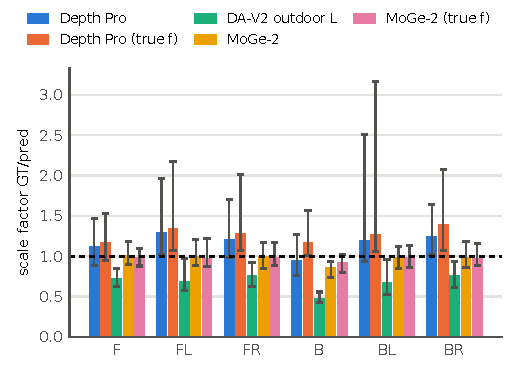
\includegraphics[width=\linewidth]{scale_per_camera.pdf}
  \caption{Median per-image scale factor GT/pred per camera (whiskers p10 to p90; dashed line: 1.0, already metric).}
  \label{fig:scale}
\end{subfigure}\hfill
\begin{subfigure}[t]{0.49\textwidth}
  \centering
  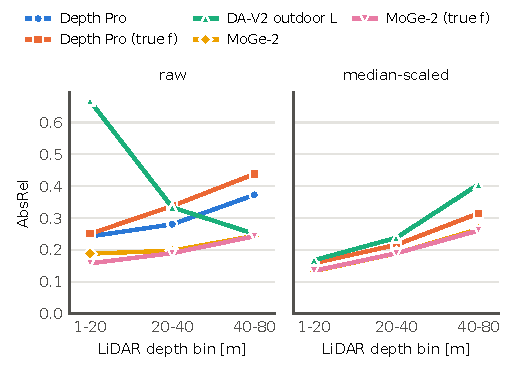
\includegraphics[width=\linewidth]{absrel_bins.pdf}
  \caption{AbsRel per depth bin, raw and median-scaled. The two Depth Pro variants coincide after scaling by construction.}
  \label{fig:bins}
\end{subfigure}
\caption{Track A: where the metric scale is off (a) and how the error changes with distance (b). Cameras: F front, FL/FR front left/right, B back, BL/BR back left/right.}
\label{fig:track_a}
\end{figure}

\paragraph{Scale and focal length.}
Figure~\ref{fig:scale} and Table~\ref{tab:track_a_scale} show the median scale factor per camera. With its
own focal estimate, Depth Pro predicts depths that are too near on the five long-focal cameras (scale
\DPscaleNonBackMin{} to \DPscaleNonBackMax{}) and close to metric on the back camera (\DPscaleBack). Its
focal estimate is above the true nuScenes focal on every camera, by a factor of \DPfocalRatioMin{} to
\DPfocalRatioMax. The largest ratio is on the back camera, whose true focal (\DPfocalTrueBack{} px) is
shorter than that of the other five (about \DPfocalTrueFront{} px). We expected the true focal to help. It
does not: AbsRel rises from \DPabsrelRaw{} to \GTFabsrelRaw{} and $\delta_1$ falls from \DPdOneRaw{} to
\GTFdOneRaw, while the median-scaled numbers are identical by construction. The scale column explains why.
With the true focal the scale factor is similar on all six cameras (\GTFscaleMin{} to \GTFscaleMax), which
means that the model's canonical depth is consistently too near on this data and that its over-estimated
focal cancels part of that. MoGe-2 behaves the way one would expect. Its focal estimate is between
\MOGEfocalRatioMin{} and \MOGEfocalRatioMax{} times the true focal, its scale factors lie between
\MOGEscaleMin{} and \MOGEscaleMax, and the true focal lowers its raw AbsRel from \MOGEabsrelRaw{} to
\MOGEGTFabsrelRaw. Depth Anything V2 metric outdoor, fine-tuned on Virtual KITTI, predicts too far on every
camera (scale \DAVscaleMin{} to \DAVscaleMax, lowest on the back camera with \DAVscaleBack).

\begin{table}[t]
\centering
\begin{subtable}[t]{\textwidth}
\centering
\adjustbox{max width=0.8\textwidth}{\footnotesize\renewcommand{\arraystretch}{0.92}
\begin{tabular}{llrrrrrr}
\toprule
model & quantity & F & FL & FR & B & BL & BR \\
\midrule
nuScenes calibration & true focal [px] & 1266 & 1273 & 1261 & 809 & 1257 & 1260 \\
\midrule
Depth Pro & median scale GT/pred & 1.122 & 1.298 & 1.212 & 0.943 & 1.195 & 1.249 \\
 & pred/true focal & 1.046 & 1.039 & 1.092 & 1.276 & 1.087 & 1.123 \\
Depth Pro (true f) & median scale GT/pred & 1.165 & 1.342 & 1.287 & 1.169 & 1.267 & 1.390 \\
DA-V2 outdoor L & median scale GT/pred & 0.728 & 0.685 & 0.757 & 0.474 & 0.677 & 0.765 \\
MoGe-2 & median scale GT/pred & 1.012 & 0.993 & 0.995 & 0.855 & 0.982 & 0.989 \\
 & pred/true focal & 0.958 & 0.974 & 0.998 & 1.225 & 1.010 & 0.992 \\
MoGe-2 (true f) & median scale GT/pred & 0.984 & 0.970 & 0.984 & 0.923 & 0.988 & 0.974 \\
\bottomrule
\end{tabular}
}
\caption{Median per-image scale factor GT/pred and focal estimate over true focal. A scale of 1.0 means the metric output is already on the LiDAR scale.}
\label{tab:track_a_scale}
\end{subtable}\\[4pt]
\begin{subtable}[t]{\textwidth}
\centering
\adjustbox{max width=0.8\textwidth}{\footnotesize\renewcommand{\arraystretch}{0.92}
\begin{tabular}{lrrrrrr}
\toprule
model & F & FL & FR & B & BL & BR \\
\midrule
Depth Pro & 0.191 / 0.124 & 0.286 / 0.182 & 0.237 / 0.204 & 0.259 / 0.177 & 0.301 / 0.174 & 0.251 / 0.202 \\
Depth Pro (true f) & 0.202 / 0.124 & 0.310 / 0.182 & 0.275 / 0.204 & 0.236 / 0.177 & 0.326 / 0.174 & 0.309 / 0.202 \\
DA-V2 outdoor L & 0.399 / 0.140 & 0.514 / 0.202 & 0.432 / 0.215 & 1.034 / 0.191 & 0.542 / 0.190 & 0.412 / 0.223 \\
MoGe-2 & 0.122 / 0.112 & 0.169 / 0.161 & 0.175 / 0.179 & 0.289 / 0.140 & 0.195 / 0.152 & 0.169 / 0.164 \\
MoGe-2 (true f) & 0.128 / 0.123 & 0.175 / 0.163 & 0.161 / 0.178 & 0.190 / 0.134 & 0.189 / 0.150 & 0.153 / 0.166 \\
\bottomrule
\end{tabular}
}
\caption{AbsRel raw / median-scaled.}
\label{tab:track_a_per_camera}
\end{subtable}
\caption{Track A per camera (F front, FL/FR front left/right, B back, BL/BR back left/right).}
\label{tab:track_a_cam}
\end{table}

\paragraph{Cameras and distance.}
The front camera is the easiest for all three models, raw and scaled, and after scaling the side cameras
are the hardest (Tables~\ref{tab:track_a_groups} and~\ref{tab:track_a_per_camera}). Depth Pro has a scaled
AbsRel of \DPabsrelFrontScaled{} on the front group and \DPabsrelSideScaled{} on the side group, Depth
Anything V2 has \DAVabsrelFrontScaled{} and \DAVabsrelSideScaled{}, and MoGe-2 has \MOGEabsrelFrontScaled{}
and \MOGEabsrelSideScaled. Before scaling the picture is mixed. Depth Pro is again worst on the side group
(\DPabsrelSideRaw{} against \DPabsrelFrontRaw{} on the front), but Depth Anything V2 and MoGe-2 are worst
on the back camera (\DAVabsrelBackRaw{} and \MOGEabsrelBackRaw), where their scale is furthest off. Errors
grow with distance (Figure~\ref{fig:bins}, Table~\ref{tab:track_a_bins}). Depth Pro's scaled AbsRel is
\DPabsrelNearScaled{} below 20 m, \DPabsrelMidScaled{} between 20 and 40 m and \DPabsrelFarScaled{} beyond
40 m, with RMSE from \DPrmseNearScaled{} to \DPrmseFarScaled{} m. The raw error of Depth Anything V2 is the
one exception. It falls with distance (\DAVabsrelNearRaw{} to \DAVabsrelFarRaw) because a global
over-estimate of depth hurts most where the true depth is small. After scaling it grows with distance like
the others.

\begin{table}[t]
\centering
\begin{subtable}[t]{0.49\textwidth}
\centering
\adjustbox{max width=\linewidth,valign=t}{\footnotesize\renewcommand{\arraystretch}{0.92}
\begin{tabular}{llrrrrr}
\toprule
model & group & AbsRel raw & scaled & $\delta_1$ raw & scaled & points \\
\midrule
Depth Pro & front & 0.191 & 0.124 & 0.633 & 0.845 & 1,219,883 \\
 & side & 0.270 & 0.190 & 0.495 & 0.739 & 5,715,488 \\
 & back & 0.259 & 0.177 & 0.549 & 0.771 & 1,826,681 \\
Depth Pro (true f) & front & 0.202 & 0.124 & 0.595 & 0.845 & 1,219,883 \\
 & side & 0.306 & 0.190 & 0.411 & 0.739 & 5,715,488 \\
 & back & 0.236 & 0.177 & 0.525 & 0.771 & 1,826,681 \\
DA-V2 outdoor L & front & 0.399 & 0.140 & 0.242 & 0.821 & 1,219,883 \\
 & side & 0.477 & 0.207 & 0.222 & 0.697 & 5,715,488 \\
 & back & 1.034 & 0.191 & 0.097 & 0.699 & 1,826,681 \\
MoGe-2 & front & 0.122 & 0.112 & 0.860 & 0.880 & 1,219,883 \\
 & side & 0.178 & 0.163 & 0.779 & 0.790 & 5,715,488 \\
 & back & 0.289 & 0.140 & 0.493 & 0.843 & 1,826,681 \\
MoGe-2 (true f) & front & 0.128 & 0.123 & 0.889 & 0.860 & 1,219,883 \\
 & side & 0.170 & 0.164 & 0.809 & 0.790 & 5,715,488 \\
 & back & 0.190 & 0.134 & 0.769 & 0.847 & 1,826,681 \\
\bottomrule
\end{tabular}
}
\caption{Per camera group (front: F; side: FL, FR, BL, BR; back: B).}
\label{tab:track_a_groups}
\end{subtable}\hfill
\begin{subtable}[t]{0.49\textwidth}
\centering
\adjustbox{max width=\linewidth,valign=t}{\footnotesize\renewcommand{\arraystretch}{0.92}
\begin{tabular}{llrrrrr}
\toprule
model & bin & AbsRel raw & scaled & RMSE raw & scaled & points \\
\midrule
Depth Pro & 1-20 m & 0.242 & 0.158 & 3.52 & 2.99 & 6,653,105 \\
 & 20-40 m & 0.280 & 0.216 & 10.22 & 8.81 & 1,599,744 \\
 & 40-80 m & 0.373 & 0.315 & 23.38 & 20.43 & 509,203 \\
Depth Pro (true f) & 1-20 m & 0.250 & 0.158 & 3.58 & 2.99 & 6,653,105 \\
 & 20-40 m & 0.338 & 0.216 & 11.55 & 8.81 & 1,599,744 \\
 & 40-80 m & 0.438 & 0.315 & 26.08 & 20.43 & 509,203 \\
DA-V2 outdoor L & 1-20 m & 0.668 & 0.168 & 6.96 & 2.50 & 6,653,105 \\
 & 20-40 m & 0.334 & 0.238 & 12.10 & 9.21 & 1,599,744 \\
 & 40-80 m & 0.250 & 0.405 & 16.98 & 24.62 & 509,203 \\
MoGe-2 & 1-20 m & 0.188 & 0.133 & 2.82 & 2.49 & 6,653,105 \\
 & 20-40 m & 0.198 & 0.189 & 8.22 & 8.28 & 1,599,744 \\
 & 40-80 m & 0.244 & 0.265 & 17.56 & 18.46 & 509,203 \\
MoGe-2 (true f) & 1-20 m & 0.158 & 0.134 & 2.62 & 2.51 & 6,653,105 \\
 & 20-40 m & 0.190 & 0.189 & 8.11 & 8.29 & 1,599,744 \\
 & 40-80 m & 0.243 & 0.261 & 17.57 & 18.29 & 509,203 \\
\bottomrule
\end{tabular}
}
\caption{Per LiDAR depth bin (RMSE in m).}
\label{tab:track_a_bins}
\end{subtable}
\caption{Track A broken down by camera group and by depth bin, raw and median-scaled, with the number of LiDAR points.}
\label{tab:track_a_breakdown}
\end{table}

\subsection{Track B: feed-forward multi-view reconstruction versus the monocular prior}
\label{sec:track_b}

\begin{table}[t]
\centering
\caption{Track B: AbsRel, $\delta_1$ and RMSE on the LiDAR pixels of the reference view, mean over \BRignSeq{} sequences per setting with 95\% bootstrap intervals. VGGT and Depth Pro are scored on identical pixels.}
\label{tab:track_b}
\adjustbox{max width=0.85\textwidth,center}{\footnotesize\renewcommand{\arraystretch}{0.92}
\begin{tabular}{lrrr}
\toprule
alignment / model & AbsRel [95\% CI] & $\delta_1$ & RMSE [m] \\
\midrule
\multicolumn{4}{l}{\emph{(i) 6-camera rig, one timestamp, reference CAM\_FRONT}} \\
VGGT raw (relative scale) & 0.901 [0.898, 0.903] &  &  \\
VGGT, one scale per sequence & 0.135 [0.120, 0.149] & 0.818 [0.787, 0.848] & 6.80 [6.08, 7.57] \\
VGGT, sim(3) scale from cameras & 0.607 [0.517, 0.699] &  &  \\
VGGT, per-image median scale & 0.124 [0.108, 0.140] & 0.854 [0.828, 0.880] & 6.35 [5.64, 7.10] \\
Depth Pro raw (metric) & 0.188 [0.166, 0.211] &  &  \\
Depth Pro, per-image median scale & 0.135 [0.116, 0.161] & 0.821 [0.767, 0.863] & 6.74 [6.12, 7.36] \\
Depth Pro raw, true focal & 0.200 [0.178, 0.223] &  &  \\
\midrule
\multicolumn{4}{l}{\emph{(ii) 5 consecutive CAM\_FRONT keyframes, reference = centre frame}} \\
VGGT raw (relative scale) & 0.901 [0.898, 0.904] &  &  \\
VGGT, one scale per sequence & 0.118 [0.097, 0.146] & 0.867 [0.818, 0.903] & 5.88 [5.18, 6.68] \\
VGGT, sim(3) scale from cameras & 0.321 [0.208, 0.452] &  &  \\
VGGT, per-image median scale & 0.123 [0.100, 0.153] & 0.862 [0.808, 0.902] & 5.93 [5.19, 6.74] \\
Depth Pro raw (metric) & 0.186 [0.162, 0.211] &  &  \\
Depth Pro, per-image median scale & 0.128 [0.112, 0.151] & 0.831 [0.778, 0.872] & 6.45 [5.88, 7.07] \\
Depth Pro raw, true focal & 0.191 [0.170, 0.214] &  &  \\
\bottomrule
\end{tabular}
}
\end{table}

VGGT is not metric. Its raw depth is off by a large constant factor (median sequence scale
\BRigscaleSeqMedian{} for the rig and \BTempscaleSeqMedian{} for the temporal window, raw AbsRel
\BRigVggtRawabsrel), so we only compare after alignment (Table~\ref{tab:track_b}). With one scale per
sequence VGGT reaches an AbsRel of \BRigVggtSeqabsrel{} on the rig and \BTempVggtSeqabsrel{} on the
temporal window. Depth Pro with its per-image median scale reaches \BRigDpImgabsrel{} and
\BTempDpImgabsrel{} on the same pixels. The paired difference, VGGT minus Depth Pro so that negative values
favour VGGT, is \BRigpairedSeq{} for the rig and \BTemppairedSeq{} for the temporal window, and both
intervals include zero. If VGGT also gets a per-image scale, the differences are \BRigpairedImg{} and
\BTemppairedImg. VGGT is ahead on average and in \BTempfracVggtLower\% of the temporal sequences, while the
rig is a tie (VGGT lower in \BRigfracVggtLower\%). On this data, then, multi-view context does not beat a
good monocular prior by a margin that a sample of this size can resolve. The monocular reference in this
track is Depth Pro. MoGe-2, which is more accurate than Depth Pro in Track A, was not run on these
sequences, so the comparison is not against the best monocular model we tested. Scaling VGGT with the similarity
transform fitted to its camera centres works much worse (\BRigVggtSimabsrel{} and \BTempVggtSimabsrel).
The baselines are short (mean \BRigbaselineMean{} m inside the rig, \BTempbaselineMean{} m between
keyframes), so the fitted scale is noisy.

\begin{table}[t]
\centering
\adjustbox{max width=\textwidth}{\footnotesize\renewcommand{\arraystretch}{0.92}
\begin{tabular}{lrrrrrrrr}
\toprule
setting & pairs & rot mean & rot median & trans mean & trans median & excluded & baseline [m] & seq. scale \\
\midrule
(i) rig & 200 & 8.12 & 4.65 & 48.6 & 35.9 & 0 & 0.81 & 23.4 \\
(ii) temporal & 160 & 0.31 & 0.14 & 2.3 & 2.0 & 40 & 4.24 & 29.7 \\
\bottomrule
\end{tabular}
}
\caption{Relative pose of VGGT against nuScenes ego poses and calibration: rotation error and translation direction error in degrees. Translation direction is evaluated only where the true baseline exceeds \BTempminBaseline{} m; ``excluded'' counts the stationary pairs; ``seq. scale'' is the median sequence scale factor.}
\label{tab:track_b_pose}
\end{table}

\paragraph{Poses.}
Table~\ref{tab:track_b_pose} gives the relative pose errors. On the temporal window VGGT's relative
rotations are accurate (median \BTemprotMedian{} degrees, mean \BTemprotMean) and the translation
directions are good too (median \BTemptransMedian{} degrees over the \BTempnPairsBaseline{} moving pairs,
with \BTempnPairsExcluded{} stationary pairs excluded). On the six-camera rig the rotations are off by
several degrees (median \BRigrotMedian, mean \BRigrotMean) and the translation directions are poor (median
\BRigtransMedian{} degrees). The nuScenes cameras overlap very little, so this is not surprising.

\subsection{Track C: 3D Gaussian Splatting on one driving scene}
\label{sec:track_c}

\begin{table}[t]
\centering
\begin{subtable}[t]{\textwidth}
\centering
\adjustbox{max width=\textwidth}{\footnotesize\renewcommand{\arraystretch}{0.92}
\begin{tabular}{llrrrrrrrrrr}
\toprule
variant & steps & PSNR & PSNR, seeds & LPIPS, seeds & SSIM & LPIPS & init & final & train min & ms/view & PSNR train \\
\midrule
random init & 7k & 13.40 $\pm$ 3.78 & 13.78 $\pm$ 0.42 (n=3) & 0.744 $\pm$ 0.012 & 0.521 & 0.758 & 200,000 & 206,811 & 1.5 & 1.9 & 20.01 \\
LiDAR init & 7k & 16.29 $\pm$ 2.75 & 15.91 $\pm$ 0.37 (n=3) & 0.590 $\pm$ 0.009 & 0.587 & 0.580 & 300,000 & 576,114 & 2.9 & 3.5 & 21.24 \\
LiDAR init + depth (w=0.05) & 7k & 17.54 $\pm$ 2.66 & 17.46 $\pm$ 0.10 (n=3) & 0.522 $\pm$ 0.003 & 0.599 & 0.525 & 300,000 & 674,323 & 3.3 & 3.9 & 21.66 \\
LiDAR init + depth (w=0.2) & 7k & 18.51 $\pm$ 2.77 & 18.43 $\pm$ 0.07 (n=3) & 0.498 $\pm$ 0.001 & 0.608 & 0.497 & 300,000 & 736,227 & 3.5 & 4.2 & 21.48 \\
\midrule
random init & 15k & 12.36 $\pm$ 2.45 & not measured & not measured & 0.512 & 0.729 & 200,000 & 427,153 & 4.4 & 2.6 & 20.61 \\
LiDAR init & 15k & 14.04 $\pm$ 3.42 & not measured & not measured & 0.522 & 0.605 & 300,000 & 948,796 & 8.4 & 5.0 & 22.44 \\
LiDAR init + depth (w=0.05) & 15k & 16.94 $\pm$ 2.79 & not measured & not measured & 0.574 & 0.469 & 300,000 & 1,337,190 & 11.6 & 7.2 & 23.43 \\
LiDAR init + depth (w=0.2) & 15k & 18.32 $\pm$ 2.63 & not measured & not measured & 0.584 & 0.417 & 300,000 & 1,516,755 & 12.8 & 8.3 & 23.32 \\
\bottomrule
\end{tabular}
}
\caption{Held-out metrics, number of Gaussians (initial and final), training minutes and render time per view on the \gpu{}. PSNR is mean $\pm$ standard deviation over views for seed 0; ``PSNR train'' is on a subset of training views. \GSseedCaption}
\label{tab:track_c}
\end{subtable}
\caption{Track C ablation on \GSscene{}, \GStestViews{} held-out views at \GSimageW$\times$\GSimageH, \gpu{}.}
\label{tab:track_c_all}
\end{table}

Table~\ref{tab:track_c} and Figure~\ref{fig:gs} show the ablation. The order of the variants is the same
at both step budgets. Random initialisation is worst (\GSRandpsnr{} dB at 7k). Aggregated LiDAR
initialisation is better on all three metrics (\GSLidarpsnr{} dB, a gain of \GSdeltaLidarRandom{} dB).
Depth supervision from the scale-aligned Depth Pro maps improves held-out PSNR, SSIM and LPIPS again, and
the larger weight does better: \GSDepthLopsnr{} dB at weight 0.05 (\GSdeltaDepthLoPsnr{} dB and
\GSdeltaDepthLoLpips{} LPIPS over LiDAR initialisation) and \GSDepthHipsnr{} dB at weight 0.2
(\GSdeltaDepthHiPsnr{} dB and \GSdeltaDepthHiLpips{} LPIPS). The 15k runs keep this order
(\GSRandFifteenKpsnr, \GSLidarFifteenKpsnr, \GSDepthLoFifteenKpsnr{} and \GSDepthHiFifteenKpsnr{} dB), and
the best variant improves its LPIPS to \GSDepthHiFifteenKlpips. Held-out PSNR, however, is lower at 15k
than at 7k for every variant, while training-view PSNR goes up (\GSDepthHipsnrTrain{} to
\GSDepthHiFifteenKpsnrTrain{} dB for the best variant). The longer runs also end with about twice as many
Gaussians (\GSDepthHigaussians{} to \GSDepthHiFifteenKgaussians) and take \GSDepthHiFifteenKtrainMin{}
instead of \GSDepthHitrainMin{} minutes on the \gpu{}.

We repeated the 7k runs with \GSnSeeds{} seeds. The seed means are \GSRandpsnrSeedMean,
\GSLidarpsnrSeedMean, \GSDepthLopsnrSeedMean{} and \GSDepthHipsnrSeedMean{} dB, with standard deviations
between \GSDepthHipsnrSeedStd{} and \GSRandpsnrSeedStd{} dB. That spread is small against the gaps between
the variants, and the order of the four variants is the same in every seed. The 15k runs were done with seed 0 only.

The absolute quality is low for 3DGS, and the numbers should be read with that in mind. The held-out views
are 0.5 s, which is several metres, away from the nearest training views. Every camera has its own
exposure, moving people and cars are modelled as static and leave ghosts, and the training views cover the
scene only once. Training-view PSNR is far below what dense captures reach, so the model is
under-constrained rather than over-fitted.

\begin{figure}[t]
\centering
\setlength{\tabcolsep}{2pt}\renewcommand{\arraystretch}{0.9}
\begin{tabular}{cc}
\small 7k steps & \small 15k steps \\
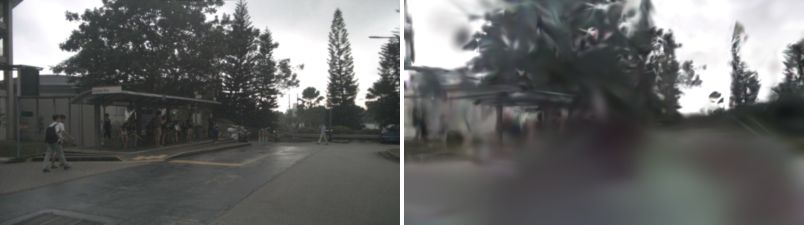
\includegraphics[width=0.27\textwidth]{gs_random_cam_front.jpg} &
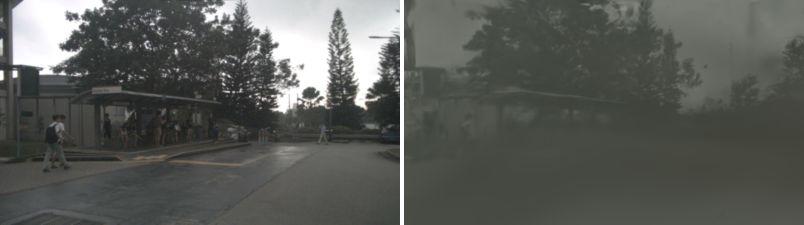
\includegraphics[width=0.27\textwidth]{gs_random_15k_cam_front.jpg} \\
\multicolumn{2}{c}{\small random initialisation} \\
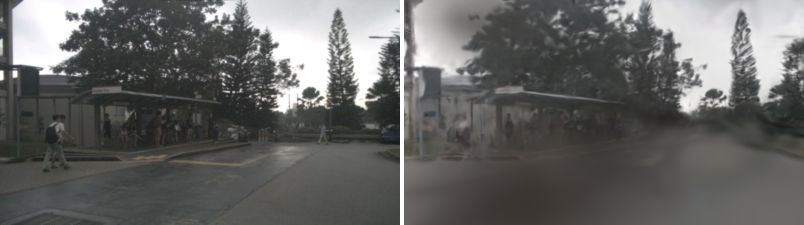
\includegraphics[width=0.27\textwidth]{gs_lidar_cam_front.jpg} &
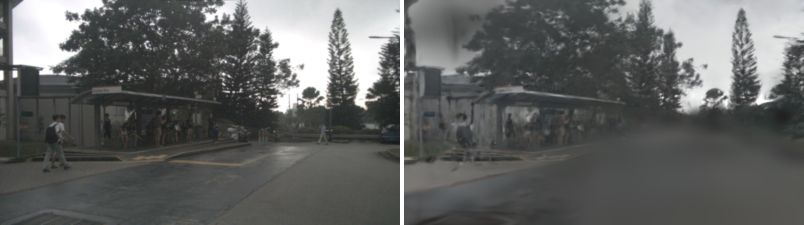
\includegraphics[width=0.27\textwidth]{gs_lidar_15k_cam_front.jpg} \\
\multicolumn{2}{c}{\small LiDAR initialisation} \\
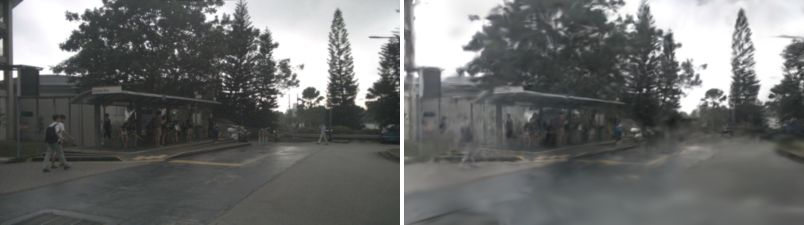
\includegraphics[width=0.27\textwidth]{gs_lidar_depth0.05_cam_front.jpg} &
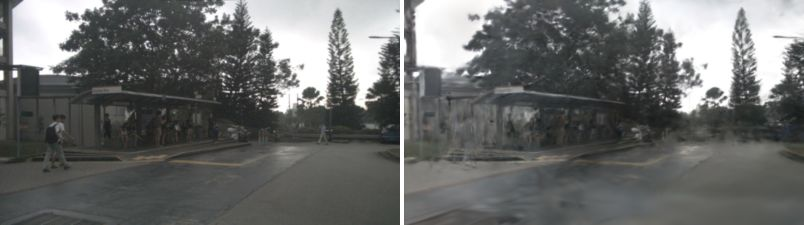
\includegraphics[width=0.27\textwidth]{gs_lidar_depth0.05_15k_cam_front.jpg} \\
\multicolumn{2}{c}{\small LiDAR initialisation + depth supervision, weight 0.05} \\
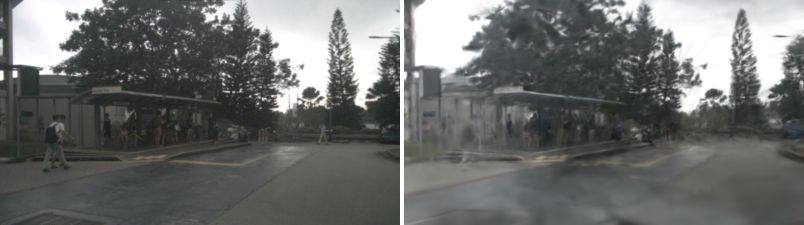
\includegraphics[width=0.27\textwidth]{gs_lidar_depth0.2_cam_front.jpg} &
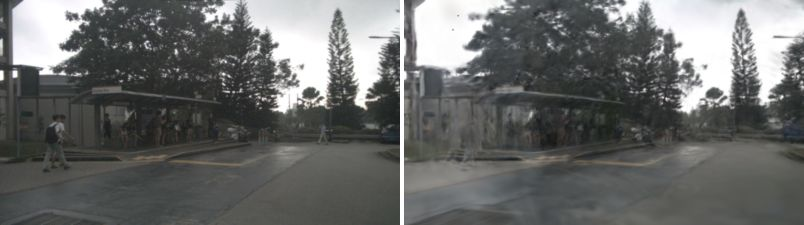
\includegraphics[width=0.27\textwidth]{gs_lidar_depth0.2_15k_cam_front.jpg} \\
\multicolumn{2}{c}{\small LiDAR initialisation + depth supervision, weight 0.2} \\
\end{tabular}
\caption{Track C, held-out CAM\_FRONT view of the first held-out timestamp, seed 0. Each panel shows the real frame (left) and the render (right). nuScenes images, CC BY-NC-SA 4.0.}
\label{fig:gs}
\end{figure}

\subsection{Track D: single-image Gaussians rendered at the true next pose}
\label{sec:track_d}

\begin{table}[t]
\centering
\begin{subtable}[t]{\textwidth}
\centering
\adjustbox{max width=0.85\textwidth}{\footnotesize\renewcommand{\arraystretch}{0.92}
\begin{tabular}{lrrrrr}
\toprule
target pose & PSNR [95\% CI] & SSIM [95\% CI] & LPIPS [95\% CI] & coverage & motion [m] \\
\midrule
identity (input pose) & 41.62 [40.69, 42.52] & 0.991 [0.987, 0.995] & 0.017 [0.014, 0.020] & 1.00 & 0.00 \\
next 12 Hz sweep & 26.80 [24.70, 28.87] & 0.773 [0.683, 0.858] & 0.096 [0.071, 0.122] & 1.00 & 0.48 \\
next keyframe & 20.42 [18.71, 22.09] & 0.592 [0.501, 0.684] & 0.231 [0.179, 0.290] & 1.00 & 2.82 \\
\bottomrule
\end{tabular}
}
\caption{Track D: SHARP Gaussians from one CAM\_FRONT keyframe per scene (\SharpImages{} images), rendered at three poses and compared with the real frame on covered pixels. Motion is the mean camera translation.}
\label{tab:track_d}
\end{subtable}\\[4pt]
\begin{subtable}[t]{\textwidth}
\centering
\adjustbox{max width=0.85\textwidth}{\footnotesize\renewcommand{\arraystretch}{0.92}
\begin{tabular}{lrrrr}
\toprule
method & PSNR [95\% CI] & LPIPS [95\% CI] & PSNR mean $\pm$ std (seeds) & LPIPS mean $\pm$ std (seeds) \\
\midrule
flow matching, one Euler sample & 23.82 [23.61, 24.04] & 0.099 [0.096, 0.102] & 23.80 $\pm$ 0.10 (n=3) & 0.098 $\pm$ 0.006 \\
regression UNet (L2) & 24.74 [24.52, 24.98] & 0.121 [0.119, 0.123] & 24.92 $\pm$ 0.19 (n=3) & 0.120 $\pm$ 0.003 \\
copy current frame & 24.38 [24.09, 24.69] & 0.040 [0.038, 0.042] & 24.38 $\pm$ 0.00 (n=3) & 0.040 $\pm$ 0.000 \\
\bottomrule
\end{tabular}
}
\caption{Track E on \NFtestPairs{} held-out pairs from scenes \NFholdoutScenes{}: PSNR and LPIPS against the real next frame. \NFseedCaption}
\label{tab:track_e}
\end{subtable}
\caption{Synthesis tracks, means with 95\% bootstrap intervals.}
\label{tab:synthesis}
\end{table}

SHARP's Gaussians re-render the input view almost perfectly (PSNR \SharpIdpsnr{} dB, LPIPS \SharpIdlpips{}
at the identity pose, Table~\ref{tab:track_d}), so the pipeline itself is sound. Quality then drops quickly
as the true camera motion grows. At the next 12 Hz sweep (\SharpSweepmotion{} m of forward motion on
average) we measure \SharpSweeppsnr{} dB and LPIPS \SharpSweeplpips, and at the next keyframe
(\SharpKeymotion{} m) \SharpKeypsnr{} dB and LPIPS \SharpKeylpips. Coverage is \SharpKeycoverage{} in both
cases, because the ego vehicle drives into the part of the scene that the Gaussians already cover.
Prediction takes \SharpPredictMs{} ms per image and a render \SharpRenderMs{} ms per view on the \gpu{}.
We did not measure where in the image the error sits. Likely sources are content that the input photo could
not see, such as the areas behind cars and poles and the road under the ego vehicle, and moving objects,
which a single-image model freezes at their position at time $t$. With ten images, one per scene, the
sample is too small to say more than this ordering. Figure~\ref{fig:sharp} shows two next-keyframe renders.

\begin{figure}[t]
\centering
\begin{subfigure}[b]{0.49\textwidth}
  \centering
  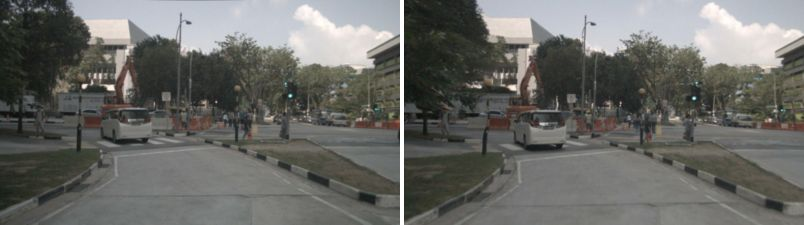
\includegraphics[width=\linewidth]{sharp_scene-0061_next_keyframe.jpg}\\[2pt]
  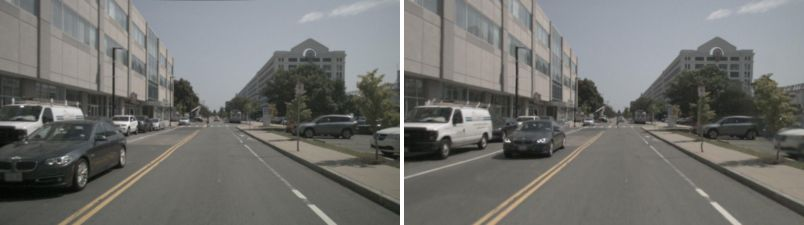
\includegraphics[width=\linewidth]{sharp_scene-0655_next_keyframe.jpg}
  \caption{Track D: real next keyframe (left) and SHARP Gaussians of the previous keyframe rendered at its true pose (right), scenes 0061 and 0655.}
  \label{fig:sharp}
\end{subfigure}\hfill
\begin{subfigure}[b]{0.49\textwidth}
  \centering
  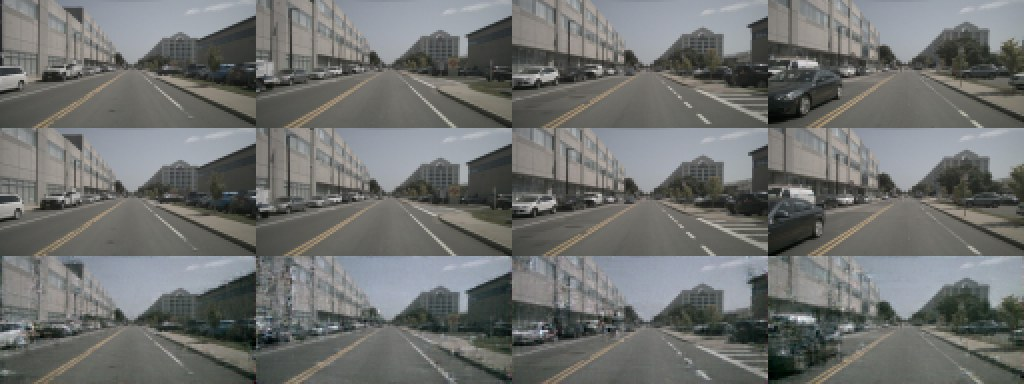
\includegraphics[width=\linewidth]{nextframe_grid.jpg}
  \caption{Track E: current frame (top row), real next frame (middle) and one flow-matching sample (bottom), four held-out pairs at \NFw$\times$\NFh.}
  \label{fig:nextframe}
\end{subfigure}
\caption{Synthesis tracks. nuScenes images, CC BY-NC-SA 4.0.}
\label{fig:synthesis}
\end{figure}

\subsection{Track E: next-frame synthesis with conditional flow matching}
\label{sec:track_e}

Table~\ref{tab:track_e} and Figure~\ref{fig:nextframe} give the result. Under the fixed
\NFFmmaxMinutes-minute budget on a shared GPU, one Euler sample from the flow-matching UNet is perceptually
closer to the real next frame than the output of the regression UNet (LPIPS \NFFmlpips{} versus
\NFReglpips, paired difference \NFpairedLpipsFmReg, interval excluding zero). Its PSNR is lower
(\NFFmpsnr{} versus \NFRegpsnr{} dB), which is the usual trade-off between a sharp sample and a blurry
mean. The copy baseline reaches \NFCopypsnr{} dB and LPIPS \NFCopylpips. The regression UNet is slightly
above it in mean PSNR but far behind in LPIPS, and the flow-matching sample is behind it on both metrics (paired
differences of \NFpairedPsnrFmCopy{} dB in PSNR and \NFpairedLpipsFmCopy{} in LPIPS). Consecutive frames
are only \NFdtMedian{} s apart, so copying is a strong baseline, and a \NFFmparams{}M-parameter model
trained for \NFFmsteps{} steps does not learn enough motion to beat it perceptually. The FID of
unconditional samples against the held-out frames is \NFfid{} (\NFfidN{} generated frames at
\NFw$\times$\NFh, upsampled for the Inception network). It is poor, and we report it only to show that the
model was not simply memorising the condition. Sampling costs \NFsamplingMs{} ms per frame on the \gpu{}.
Over \NFnSeeds{} seeds the flow-matching samples reach \NFFmpsnrSeedMean{} $\pm$ \NFFmpsnrSeedStd{} dB and
LPIPS \NFFmlpipsSeedMean{} $\pm$ \NFFmlpipsSeedStd, and the regression model \NFRegpsnrSeedMean{} $\pm$
\NFRegpsnrSeedStd{} dB and \NFReglpipsSeedMean{} $\pm$ \NFReglpipsSeedStd, so the picture does not depend
on the seed.

\subsection{Runtimes}
\label{sec:runtimes}

Table~\ref{tab:runtimes} lists every job with its wall-clock time on the \gpu{}. The Track A, B and C jobs
ran one after another on an otherwise idle GPU, with two exceptions. A few short smoke tests shared the GPU
during the Depth Pro rerun, which is why we report the median time per image, and the two Track E trainings
of each seed shared the GPU with each other.

\begin{table}[t]
\centering
\caption{Wall-clock time of every job on the \gpu{} (LiDAR projection on the CPU).}
\label{tab:runtimes}
\adjustbox{max width=0.8\textwidth,center}{\footnotesize\renewcommand{\arraystretch}{0.92}
\begin{tabular}{llr}
\toprule
job & size & minutes (NVIDIA L4) \\
\midrule
LiDAR GT projection (CPU) & 2,424 images & 0.4 \\
Track A DA-V2 outdoor L & 2,424 images, 365 ms/img median & 14.9 \\
Track A Depth Pro & 2,424 images, 599 ms/img median & 26.5 \\
Track A MoGe-2 & 2,424 images, 188 ms/img median & 8.0 \\
Track C 3DGS, 4 variants (seed 0) & 7,000 steps each, 33.3 to 77.7 steps/s & 11.5 (sum) \\
Track C 3DGS, 4 variants (seed 0) & 15,000 steps each, 19.5 to 56.2 steps/s & 37.5 (sum) \\
Track C 3DGS, additional seeds & 8 runs & 22.4 (sum) \\
Track B VGGT (+ Depth Pro on reference views) & 80 sequences & 2.0 \\
Track E train fm & 2,150 steps, 0.9 steps/s (GPU shared with the other training) & 40.0 \\
Track E train regression & 2,150 steps, 0.9 steps/s (GPU shared with the other training) & 40.0 \\
Track E training, additional seeds & 4 runs & 160.1 (sum) \\
Track E eval (sampling only) & 467 pairs, 173.8 ms/sample & 1.4 \\
Track E DDP smoke (torchrun, gloo, 2 ranks on one GPU) & 20 steps, world size 2 & 0.08 \\
Track D SHARP & 10 images, 5496 ms predict, 22.0 ms render per view & n/a \\
\bottomrule
\end{tabular}
}
\end{table}

\section{Discussion}
\label{sec:discussion}

\paragraph{Scale versus shape.}
The raw versus median-scaled split shows how much of the error one scalar per image removes on nuScenes:
\DPscaleShare\% of Depth Pro's AbsRel, \DAVscaleShare\% of Depth Anything V2's and \MOGEscaleShare\% of
MoGe-2's. Before scaling the three models are far apart (\MOGEabsrelRaw, \DPabsrelRaw{} and
\DAVabsrelRaw). After scaling they are close (\MOGEabsrelScaled, \DPabsrelScaled{} and \DAVabsrelScaled).
The models therefore differ much more in how well they guess the metric scale than in the shape they
recover, and a ranking by raw error is to a large part a ranking of the scale guess. MoGe-2 leads on both
counts here. A practical consequence is that any source of one scalar per image, for example a few LiDAR
returns, a known object size or a multi-view constraint, is worth more for Depth Pro and Depth Anything V2
than switching between the two. Track B points the same way. A multi-view model without metric scale, given
one scalar per sequence, reaches the same AbsRel as median-scaled Depth Pro on identical pixels.

\paragraph{Depth Pro and the true focal length.}
Depth Pro's depth is proportional to the focal length it uses, $d = f\,/\,(W\,c)$, where $c$ is its
canonical inverse depth. Its focal estimate is above the true nuScenes focal on every camera, most of all
on the back camera, which has the shortest true focal. Even so, the output with the model's own focal is
closer to metric than the output with the true focal. The scale factors explain this. With the true focal
all six cameras show a similar under-estimation (scale \GTFscaleMin{} to \GTFscaleMax), so the canonical
depth itself is too near on this data, and the over-estimated focal happens to compensate part of it. To
rule out a bug on our side we cross-checked the result against the library's own known-focal path (maximum
difference \FocalCheckMaxDiff{} m). For this model on this data, the correct intrinsics give a worse raw
result overall than the model's own guess. The back camera is the exception (raw AbsRel
\GTFabsrelBackRaw{} with the true focal against \DPabsrelBackRaw{} with the estimated one), because there
the estimated focal over-compensates. We cannot tell from this data which of the two effects, the canonical
depth or the focal estimate, reflects the training distribution. MoGe-2 does not show the effect. The true
focal lowers its raw AbsRel from \MOGEabsrelRaw{} to \MOGEGTFabsrelRaw.

\paragraph{Side cameras.}
After scaling, the side cameras are the hardest for all three models, and for Depth Pro they are the
hardest before scaling as well. We think the reason is content rather than optics. Side views are dominated
by close, oblique facades, parked cars and vegetation, with many LiDAR returns under 20 m
(Table~\ref{tab:lidar_gt}). This is only a hypothesis. Our data cannot separate it from a mismatch in focal
length or field of view to the training distribution. One observation speaks against a pure focal effect:
after scaling, the back camera, which has the shortest focal, is not the hardest for any of the three
models (\DPabsrelBackScaled, \DAVabsrelBackScaled{} and \MOGEabsrelBackScaled).

\paragraph{Why the geometry prior helps 3DGS.}
The capture sees the scene once, with views 0.5 s apart. In that setting the photometric loss alone does
not constrain the geometry enough, as the random-initialisation result shows. LiDAR points fix where
surfaces are, and the aligned monocular map adds a dense target where LiDAR is sparse. Within the two
weights we tested, more depth weight gives more gain, at both step budgets. The limit of the prior shows up
as well. Training longer raises training-view PSNR but not held-out PSNR, which suggests that the model is
limited by what the views constrain (exposure, moving objects and sky are not modelled) and not by the
length of the optimisation.

\paragraph{The copy-frame baseline.}
At \NFdtMedian{} s spacing and \NFw$\times$\NFh{} resolution the next frame differs from the current one
by a small motion. A copy of the current frame is therefore already close to the target in both PSNR and
LPIPS, and a generative model has to reproduce the current frame exactly and also move it correctly just to
break even. Track D shows a similar pattern. SHARP's geometry handles a \SharpSweepmotion{} m step well and
a \SharpKeymotion{} m step poorly, because the parts of the next view that the current image does not
contain have to be invented. In both tracks the quality of the synthesis ends where the geometry available
from the input ends.

\section{Limitations}
\label{sec:limits}

\begin{itemize}
  \item \textbf{Mini split only.} nuScenes-mini has 10 scenes, \GTkeyframes{} keyframes and one city pair.
        Nothing here is a claim about full nuScenes or other data.
  \item \textbf{Seeds.} The 7k 3DGS runs use \GSnSeeds{} seeds and the next-frame models \NFnSeeds{}. The
        15k 3DGS runs and the evaluations of the pretrained models were each done once. Bootstrap
        intervals over views, pairs, images or sequences do not capture seed variance.
  \item \textbf{Monocular model in Tracks B and C.} The paired comparison with VGGT and the depth
        supervision for 3DGS both use Depth Pro. MoGe-2 was added to Track A afterwards and is more
        accurate there, but Tracks B and C were not repeated with it.
  \item \textbf{Static-scene assumption.} 3DGS and SHARP treat the scene as static, so moving people and
        cars leave ghosts in every variant. We picked the most static scene for 3DGS, but it still contains
        \GSsceneMoving{} moving annotations.
  \item \textbf{Reduced resolution.} 3DGS trains and evaluates at \GSimageW$\times$\GSimageH, SHARP is
        scored at \SharpEvalW$\times$\SharpEvalH{} and Track E uses \NFw$\times$\NFh{} frames. VGGT sees
        518$\times$294 and its depth is upsampled to the LiDAR pixels.
  \item \textbf{Sparse LiDAR ground truth.} There are only \GTptsMin{} to \GTptsMax{} points per image, and
        they are biased towards the near range. Occlusion at depth discontinuities, moving objects and
        LiDAR-camera time offsets add noise that no model can remove, and z-buffering cannot remove points
        that are occluded for the camera but visible for the LiDAR.
  \item \textbf{Models as published.} The zero-shot models use their public weights and default
        preprocessing. Depth Anything V2 metric outdoor is fine-tuned on Virtual KITTI, so its scale
        reflects KITTI's camera. Depth Pro and SHARP assume the principal point at the image centre, while
        \PPsentence{}.
  \item \textbf{Fixed budgets, single machine.} 3DGS uses fixed step budgets without tuning. The Track E
        models are tiny, trained under a wall-clock cap on a shared GPU and sampled once per pair with
        plain Euler, and an FID over a few hundred small frames is only indicative. Every timing is from
        one \gpu{}, and the distributed code path was only smoke-tested on it.
\end{itemize}

\section{Conclusion}
\label{sec:conclusion}

On this driving data, zero-shot monocular depth models recover shape much better than metric scale. A
feed-forward multi-view model with one scale per sequence reaches the accuracy of median-scaled Depth Pro on
identical pixels and
also gives accurate relative rotations between consecutive frames. The scale-aligned monocular depth helps
Gaussian Splatting from sparse views. Synthesis from a single image or frame holds up only for small
changes. A pose change of \SharpSweepmotion{} m costs little and one of \SharpKeymotion{} m costs a lot,
and at \NFdtMedian{} s spacing a copy of the current frame is perceptually closer to the next frame than
our small generative model. All of this was measured on ten scenes and one GPU with few seeds, so it should
be taken as a small, checkable data point and not as a benchmark. Everything can be regenerated with the
released scripts.

\section*{Reproducibility statement}

The code, the measured json files and the scripts that write every table and macro of this report are at
\url{https://github.com/pavanyadava007/depth3d-lab}. There is one script per experiment in
\texttt{scripts/}, and the json files they write are in \texttt{results/}. \texttt{paper/make\_tables.py}
and \texttt{paper/make\_figs.py} regenerate \texttt{paper/tables/}, \texttt{paper/numbers.tex} and
\texttt{paper/figs/}, and Tectonic compiles \texttt{paper/main.tex}. The environment is Python 3.10, torch
2.7.1 with CUDA 12.6 wheels and gsplat 1.5.3 on one \gpu{} (23 GB). No number in the prose is typed by
hand. Each is a macro written by \texttt{make\_tables.py}, and a missing result file produces the words
``not measured'' instead of a value.

{\footnotesize\setlength{\bibsep}{1.5pt}
\bibliographystyle{plainnat}
\bibliography{refs}}

\end{document}
